\documentclass[12pt,a4paper]{article}
\usepackage[T1]{fontenc}
\usepackage[utf8]{inputenc}
\usepackage[margin=2cm]{geometry}
\usepackage[francais]{babel}
\usepackage{graphicx}
\usepackage{amsmath}
\usepackage{subfig}


\begin{document}
\title{Projet A.L.A.M.\\ Systèmes de recommandation DIY}
\date{\today}
\author{Louis Becquey - 3BIM}
\maketitle
\newpage

\section{Question A - Chargez les données}
Les données du site movielens.org sont chargées dans des dictionnaires python.
\section{Question B - Matrice Utilisateur-Item}
On construit une matrice R de 943 lignes (les utilisateurs) et 1682 colonnes (les films).
\begin{figure}[h!]
	\centering
	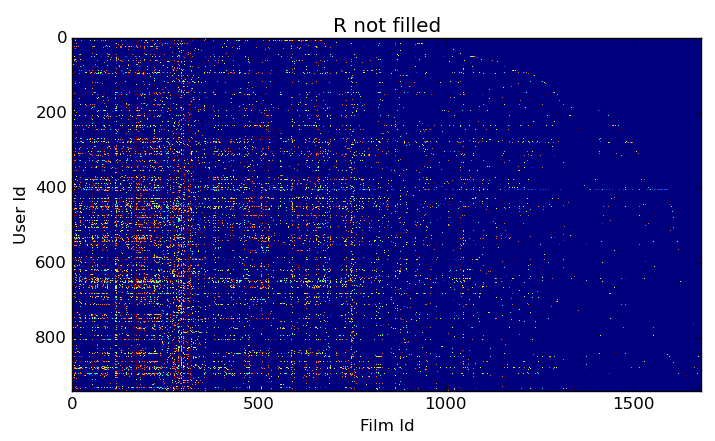
\includegraphics[scale=0.5]{R-Not-Filled.png}
	\caption{Matrice $R$ de données: Bleu=Pas de vote, couleurs du vert au rouge=note de 1 à 5 étoiles.}
\end{figure}
\\
On remarque qu'il existe des films qui n'ont été notés par personne, cependant, il n'existe pas d'utilisateur qui n'aie voté pour aucun film.
\newpage

\section{Question C - Approximation bas-rang par SVD}
On remplit les données manquantes de la matrice $R$ de deux façons différentes, en utilisant la moyenne des notes de ce film, ou en utilisant la moyenne des notes de cet utilisateur.\\

\begin{figure}[h!]
	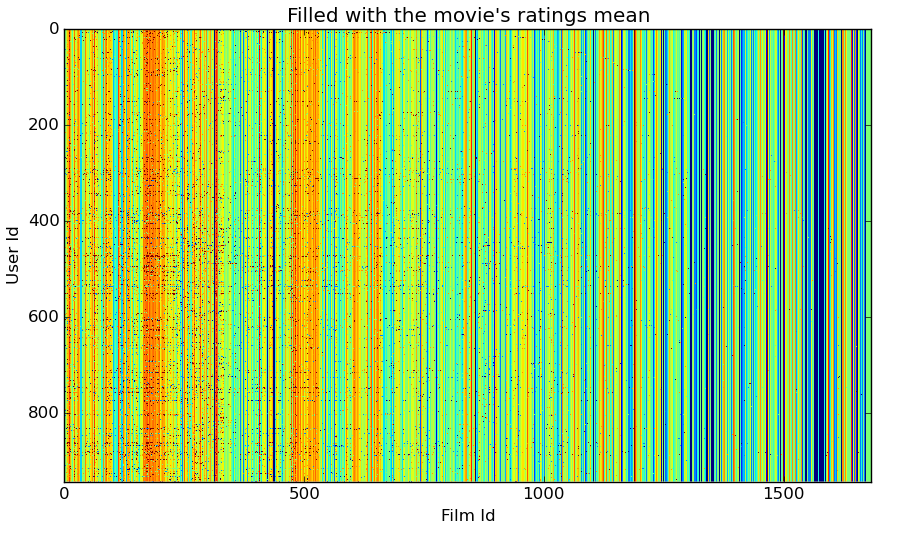
\includegraphics[scale=0.28]{R-Filled-By-Movie.png}
	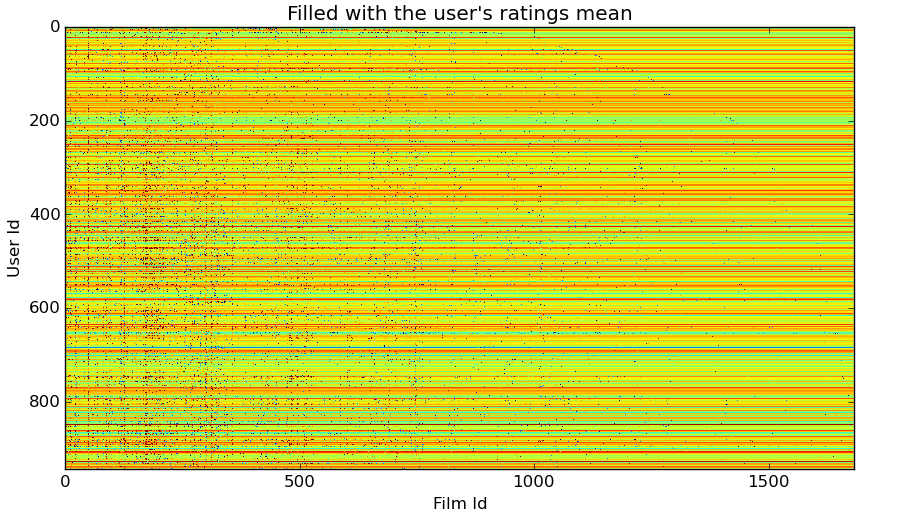
\includegraphics[scale=0.28]{R-Filled-By-User.png}
	\caption{A droite: Matrice $Rc$ remplie avec la moyenne du film lors de données manquantes. A gauche: Matrice $Rr$ remplie avec la moyenne de l'utilisateur lors de données manquantes.}
\end{figure}

On utilisera \texttt{ numpy.linalg.svd() } pour calculer les décompositions en valeurs singulières. $$R=USV'$$On réalise ensuite l'approximation de $Rc$ ou $Rr$ en ne retenant que $k$ valeurs singulières sur $m$.\\ Éliminer les $(m-k)$ dernières valeurs singulières revient à éliminer dans le calcul les valeurs des $(m-k)$ dernières colonnes de $U$ et des $(m-k)$ dernières lignes de $V'$.\\
Donc à partir de $U$ de taille $m\times m$, $S$ de taille $m \times m$ et $V'$ de taille $m \times n$, on ne garde que $U_k$ une matrice de taille $m \times k$, $S_k$ de taille $k \times k$ et $V'_k$ de taille $k \times n$.
$$R \approx U_kS_kV'_k$$

$\Rightarrow$ Comprendre Xk et Yk, et Xk(u,) et Yk(:,i)

\newpage
\section{Question D - Qualité de la prédiction par SVD}
On peut estimer l'erreur par la moyenne (en note) des différences entre la note réelle dans l'échantillon test et celle prévue par l'approximation de rang k (en valeur absolue), dite MAE (Mean Absolute Error).\\

\begin{figure}[h!]
	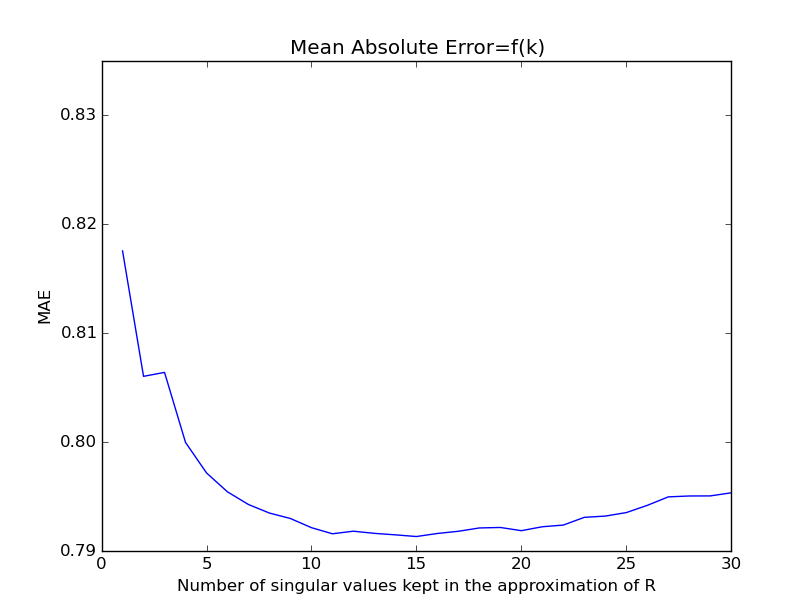
\includegraphics[scale=0.38]{MAE-By-Movie.png}
	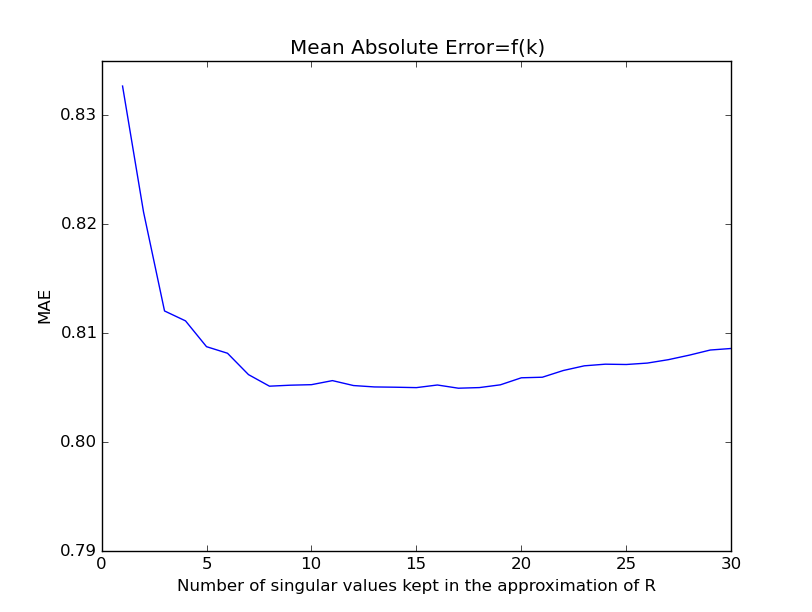
\includegraphics[scale=0.38]{MAE-By-User.png}
	\caption{A droite: MAE selon le rang de l'approximation, pour Rc (moyenne du film) à gauche, et pour Rr (moyenne de l'utilisateur) à droite.}
\end{figure}

On remarque donc que la méthode naïve utilisant la moyenne du film est légèrement plus fidèle.\\
En prenant k=12, on arrive à se limiter à une erreur d'environ 0,792 par note.\\
Il est important de se rappeler que cette note est attribuée en étoiles de 1 à 5, sans décimales. On pourrait donc arrondir l'erreur et considérer que cette méthode est précise à plus ou moins 1 étoile.\\

Si ensuite on souhaite mesurer l'erreur due à l'approximation par SVD, on peut là aussi faire la moyenne des différences (en valeur absolue) entre la matrice remplie par méthode naïve et l'approximation de cette même matrice, avec k=12.\\
On obtient, pour Rr comme pour Rc, une erreur d'environ 0,06 étoile, ce qui est faible et tout à fait satisfaisant.\\

En effet, l'approximation de la matrice permet d'\textbf{économiser énormément d'espace de stockage} (dans notre exemple: $943\times1682=1586126$ contre $943\times12+1682\times12+12\times12=31644$ soit un facteur 50). En revanche, le \textbf{temps de calcul est plus long} puisque l'on doit calculer deux produits pour obtenir le résultat. Et ceci pour une \textbf{différence de qualité de précision faible} étant donné la MAE de la méthode en général face aux réelles valeurs de l'échantillon test (0,06 contre 0,79).

\section{Question E - Théorie}
Montrons que si une matrice A est réelle, alors elle admet une décomposition en valeurs singulières $A=U \Sigma V^{*}$, avec U et V des matrices à coefficients réels.

$\Rightarrow$ Euh...

\section{Question F - Problème des moindres carrés pour méthode alternée}
On a pour objectif d'obtenir $X.Y\approx R$. Le rôle de la ligne $X_u$ dans ce produit est de permettre de calculer les valeurs de la ligne $R_u$ dans la matrice finale. Ainsi, 
$$X_u.Y\approx R_u$$
$$(X_u.Y)^T\approx (R_u)^T$$
$$Y^T.X_u^T\approx R_u^T$$
où $Y^T$ est une matrice $n\times k$, et $X_u^T$ et $R_u^T$ deux vecteurs colonnes, $R_u^T$ connu. \\
Il s'agit donc d'un problème des moindres carrés linéaire.\\

Et plus directement, le rôle de la colonne $Y_i$ est de permettre le calcul des valeurs de la colonne $R_i$, donc:
$$X.Y_i \approx R_i$$
Il s'agit là aussi d'un problème des moindres carrés linéaire.\\

Choisissons donc une matrice Y arbitraire, par exemple pleine de 1. On va donc résoudre le problème linéaire $Y^T.X_u^T= R_u^T$ pour chaque ligne $X_u$, ce qui nous donnera une matrice X. Connaissant cette matrice X, on résout le problème $X.Y_i = R_i$ pour préciser notre matrice Y. On répète ce schéma un certain nombre de fois en espérant que X et Y convergent vers une solution qui minimise l'erreur moyenne absolue. On obtient les résultats suivants:

\begin{figure}[h]
\centering
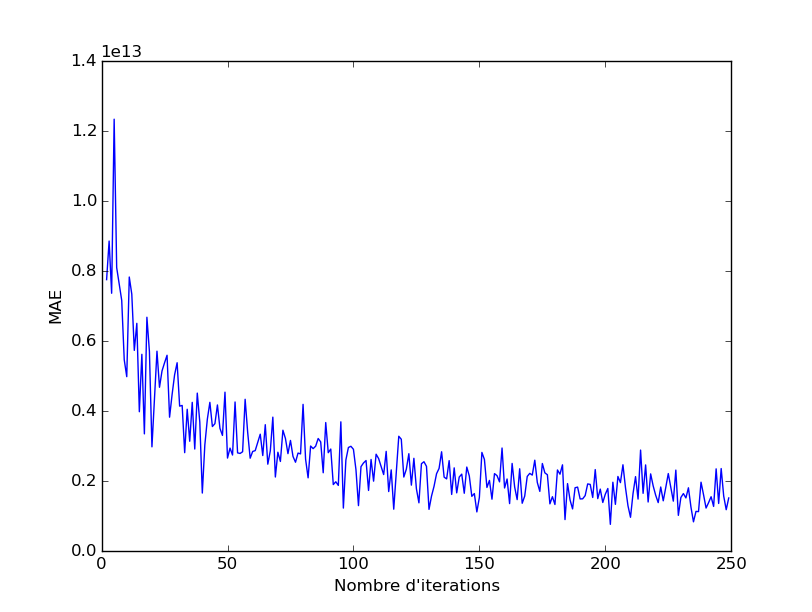
\includegraphics[scale=0.5]{least-squares-MAE.png}
\caption{Des MAE de l'ordre de $10^{12}$ pour 250 itérations...}
\end{figure}
On remarque donc que cette méthode converge, mais beaucoup trop lentement à notre goût. \textit{(Diminution d'une puissance de 10 en moyenne en 200 itérations = 10 minutes de calcul)}

\newpage
Cherchons donc plutôt des matrices X et Y de taille plus petite: $943\times k$ et $k\times 1682$.\\
Puis restreignons les calculs aux coefficients non nuls de R, et accordons nous une erreur $\lambda$ au sens des moindres carrés. On cherche donc les lignes u de X et les colonnes i de Y telles que la quantité
$$\sum_{u,i} (R_{u,i}-X_uY_i)^2+\lambda \left(\sum_u ||X_u||^2 + \sum_i ||X_i||^2 \right) \text{soit minimisée.}$$

On crée donc une matrice W de même taille que R, dont les valeurs sont 1 si $R_{u,i} \neq 0$, zéro sinon. Cela revient à minimiser les fonctions suivantes sur $X_u$ et $Y_i$ :
$$\begin{array}{l}
\text{Pour Y fixé, } F(X_u) = (R_u -X_uY) diag(W_u) (R_u -X_uY)^* + \lambda X_u X_u^*\\
\text{Pour X fixé, } G(Y_i) = (R_i -XY_i)^* diag(W_i) (R_i -XY_i) + \lambda Y_i^*Y_i\\
\end{array}$$
Le minimum local de ces deux fonctions correspondra au minimum local de la quantité ci-dessus. On cherche donc ce point, pour lequel $\frac{\partial F}{\partial X_u}=\frac{\partial G}{\partial Y_i}=0$.

$$F(X_u) = (R_u -X_uY) diag(W_u) (R_u -X_uY)^* + \lambda X_u X_u^*$$
$$F(X_u) = (R_u^* -Y^*X_u^*)^* diag(W_u) (R_u^* -Y^*X_u^*) + \lambda X_u X_u^*$$
$$0=\frac{dF(X_u)}{dX_u}=\frac{dx}{dX_u}\frac{dF}{dx}+\lambda \frac{d}{dX_u}(X_uX_u^*) \text{ avec } x=R_u^* -Y^*X_u^*$$
$$0=-Y.2.diag(W_u)(R_u^*-Y^*X_u^*)+2.\lambda.X_u^*$$
$$0=Y.diag(W_u).(Y^*X_u^*-R_u^*)+\lambda X_u^*$$
$$0=Y.diag(W_u).Y^*X_u^*-Y.diag(W_u).R_u^*+\lambda X_u^*$$
$$\text{Donc }(Y.diag(W_u).Y^*+\lambda I)X_u^* = Y.diag(W_u).R_u^*$$
\begin{center}
\fbox{$X_u=\left[ (Y.diag(W_u).Y^*+\lambda I)^{-1}.(Y.diag(W_u).R_u^*) \right]^*$}
\end{center}
Cette équation normale nous donne la capacité d'estimer X quand on connaît R, W, $\lambda$, et Y. On peut faire de même pour trouver une expression de $Y_i$:
$$G(Y_i) = (R_i -XY_i)^* diag(W_i) (R_i -XY_i) + \lambda Y_i^*Y_i$$
$$0=\frac{dG(Y_i)}{dY_i}=\frac{dx}{dY_i}\frac{dG}{dx}+\lambda \frac{d}{dY_i}(Y_i^*Y_i)\text{ avec }x=R_i-XY_i$$
$$0=-X^*.2.diag(W_i)(R_i -XY_i) + \lambda 2 Y_i$$
$$0=X^*diag(W_i)(XY_i-R_i)+\lambda Y_i$$
$$0=X^*.diag(W_i)XY_i-X^*diag(W_i)R_i+\lambda Y_i$$
$$\text{Donc }(X^*diag(W_i)X+\lambda I)Y_i=X^*diag(W_i)R_i$$
\begin{center}
\fbox{$Y_i = (X^*diag(W_i)X+\lambda I)^{-1}.(X^*diag(W_i)R_i)$}
\end{center}
On a transformé le problème des moindres carrés non linéaire en deux problèmes linéaires (\textit{de type $A.x=b$ avec A et b connus}), qu'on va résoudre par une approche itérative: prendre deux matrices X et Y arbitraires (pleines de 1), estimer X, puis estimer Y avec ce X, puis recommencer un certain nombre d'itérations en espérant converger vers des solutions minimisant la MAE:
\newpage
\begin{table}[h]
\begin{tabular}{cc}
\subfloat[Pour k=3 ; $\lambda=0.02$]{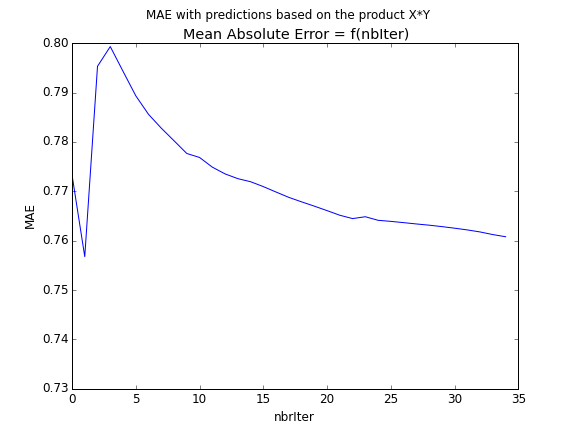
\includegraphics[scale=0.3]{MAE-least-squares-k3-l2.png}}
&
\subfloat[Pour k=3 ; $\lambda=0.80$]{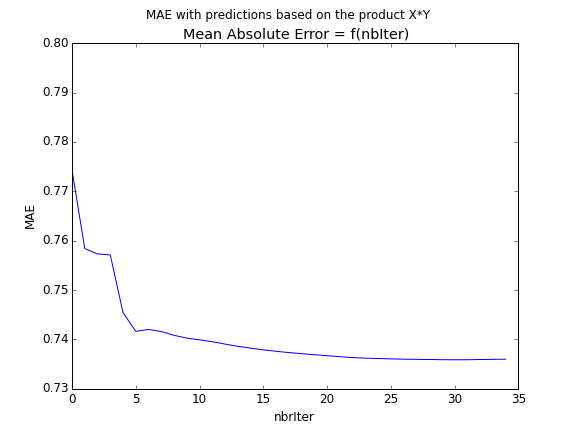
\includegraphics[scale=0.3]{MAE-least-squares-k3-l80.png}}
\end{tabular}
\end{table}

\begin{table}[h]
\begin{tabular}{cccc}
\subfloat[X*Y à la $1^{ere}$ itération]{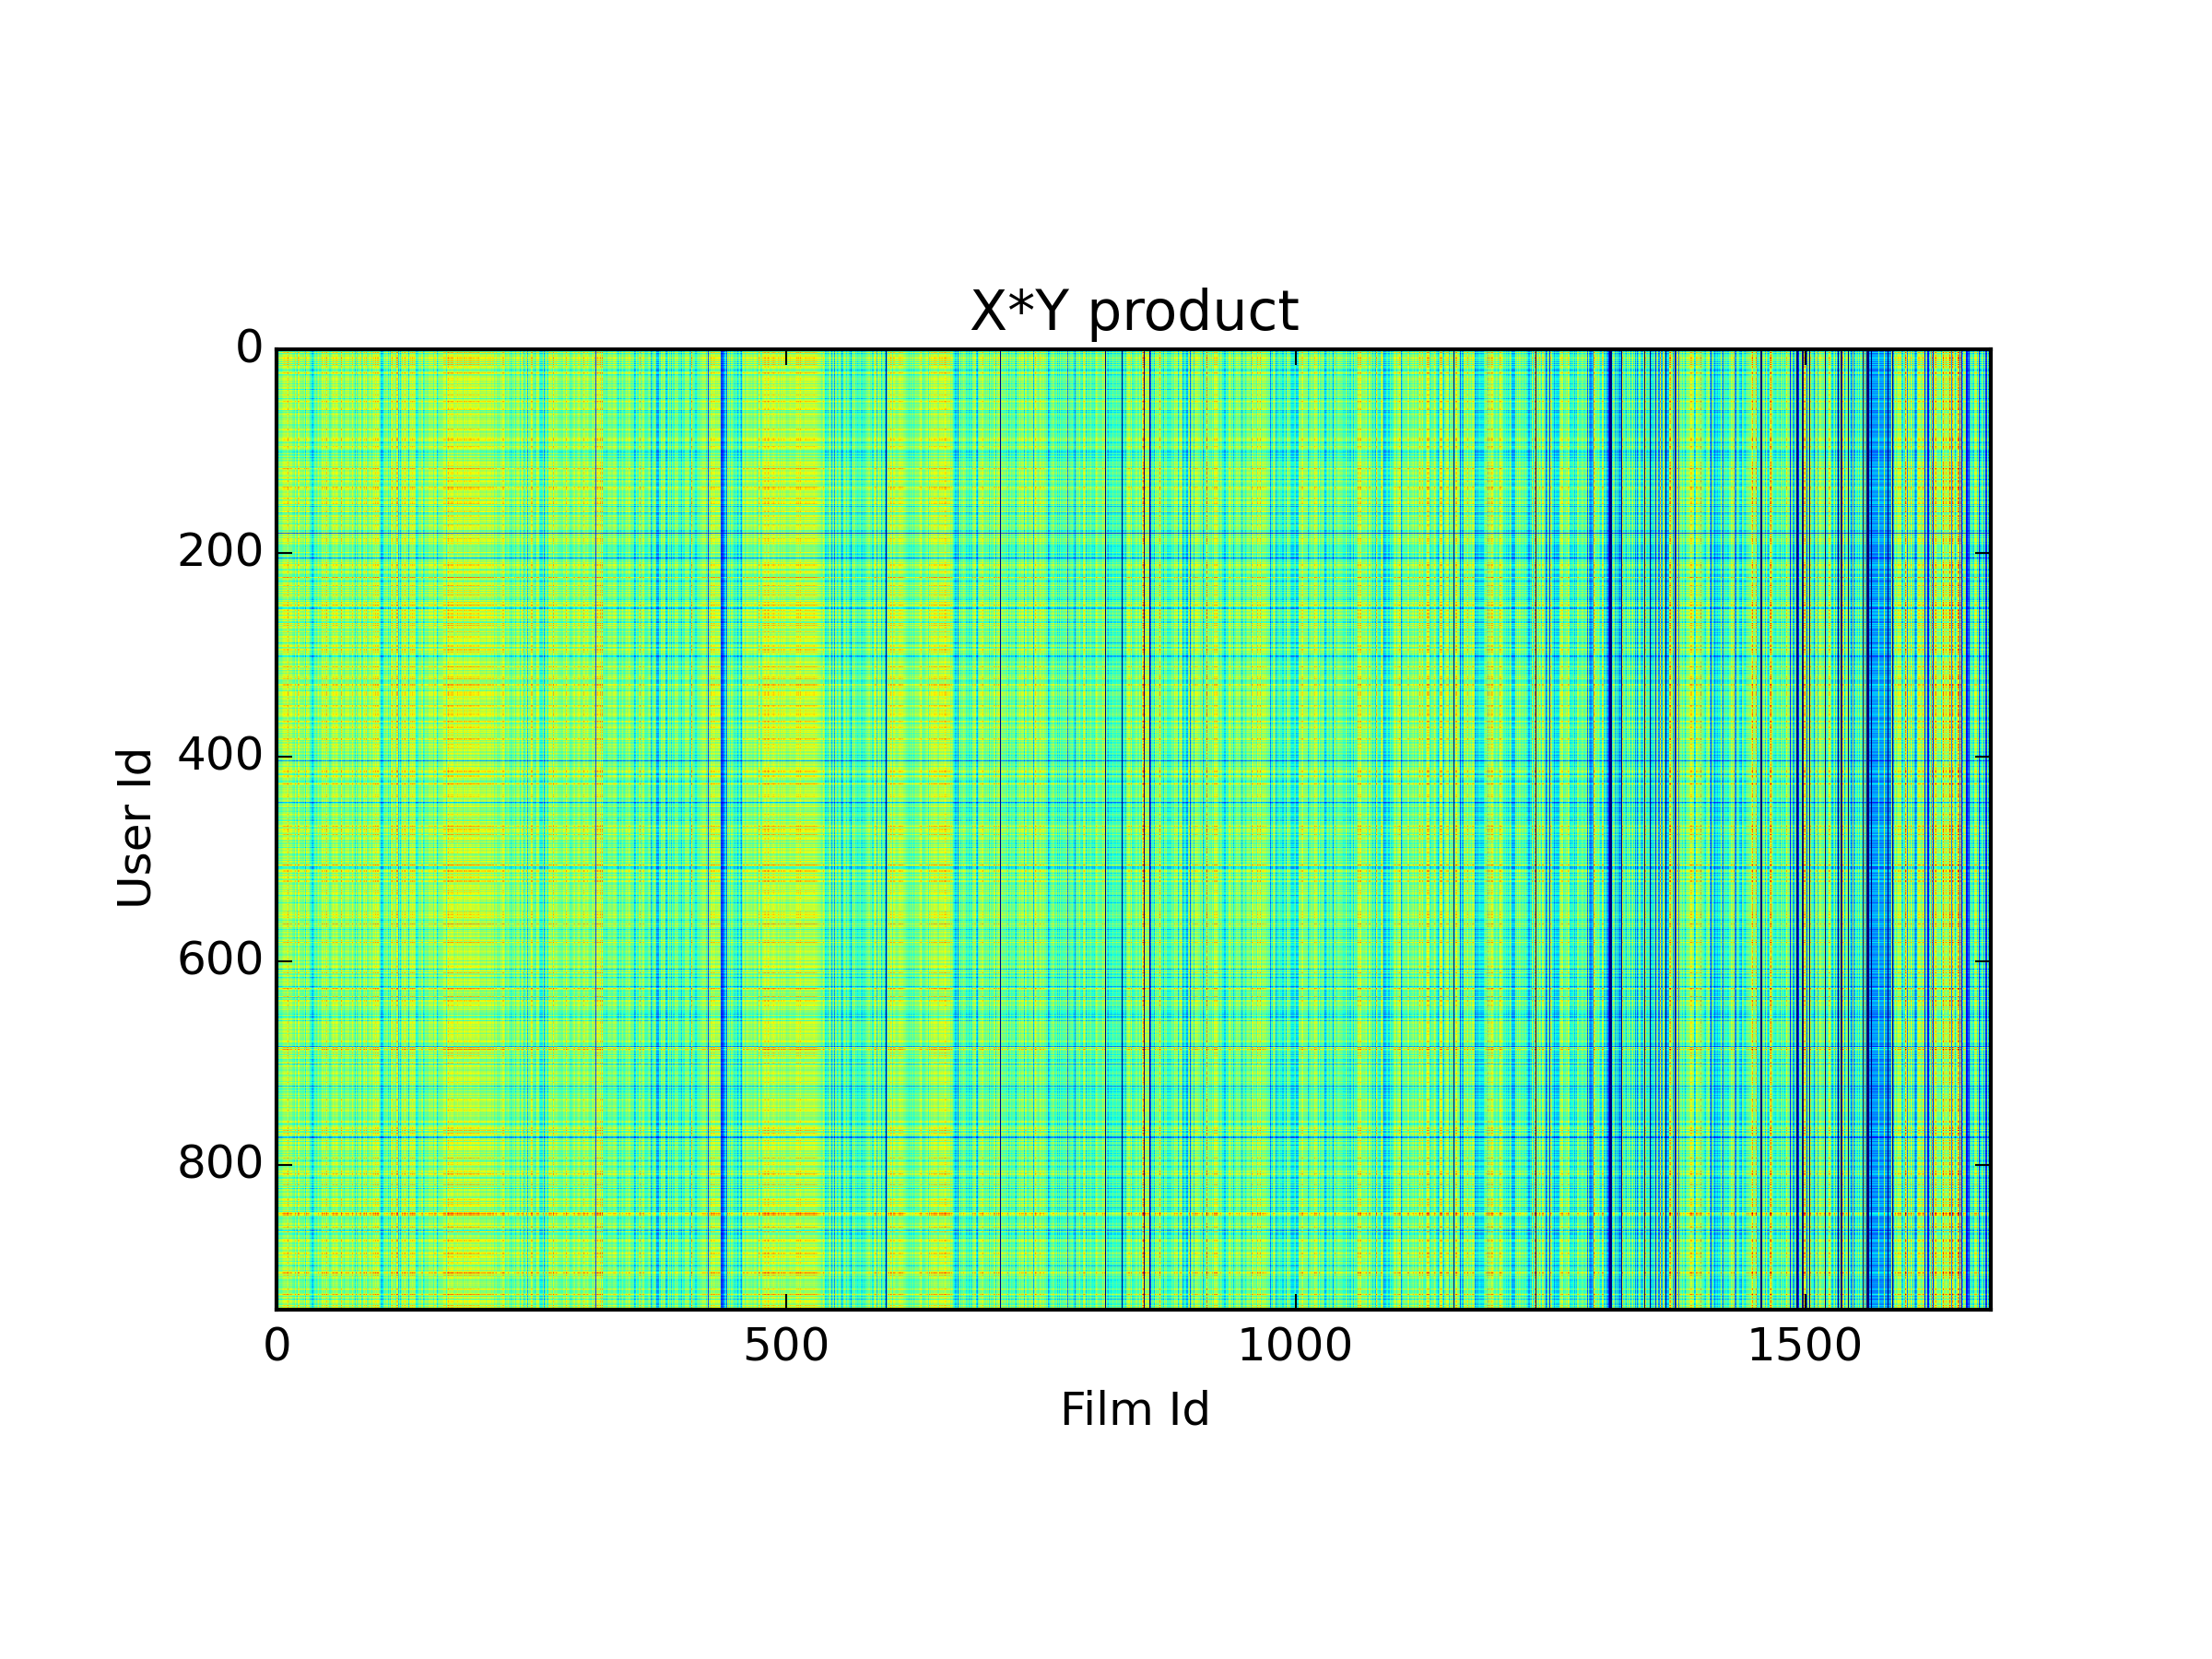
\includegraphics[scale=0.2]{it1-k3-l2.png}}
&
\subfloat[X*Y à la $2^e$ itération \textit{(meilleure MAE)}]{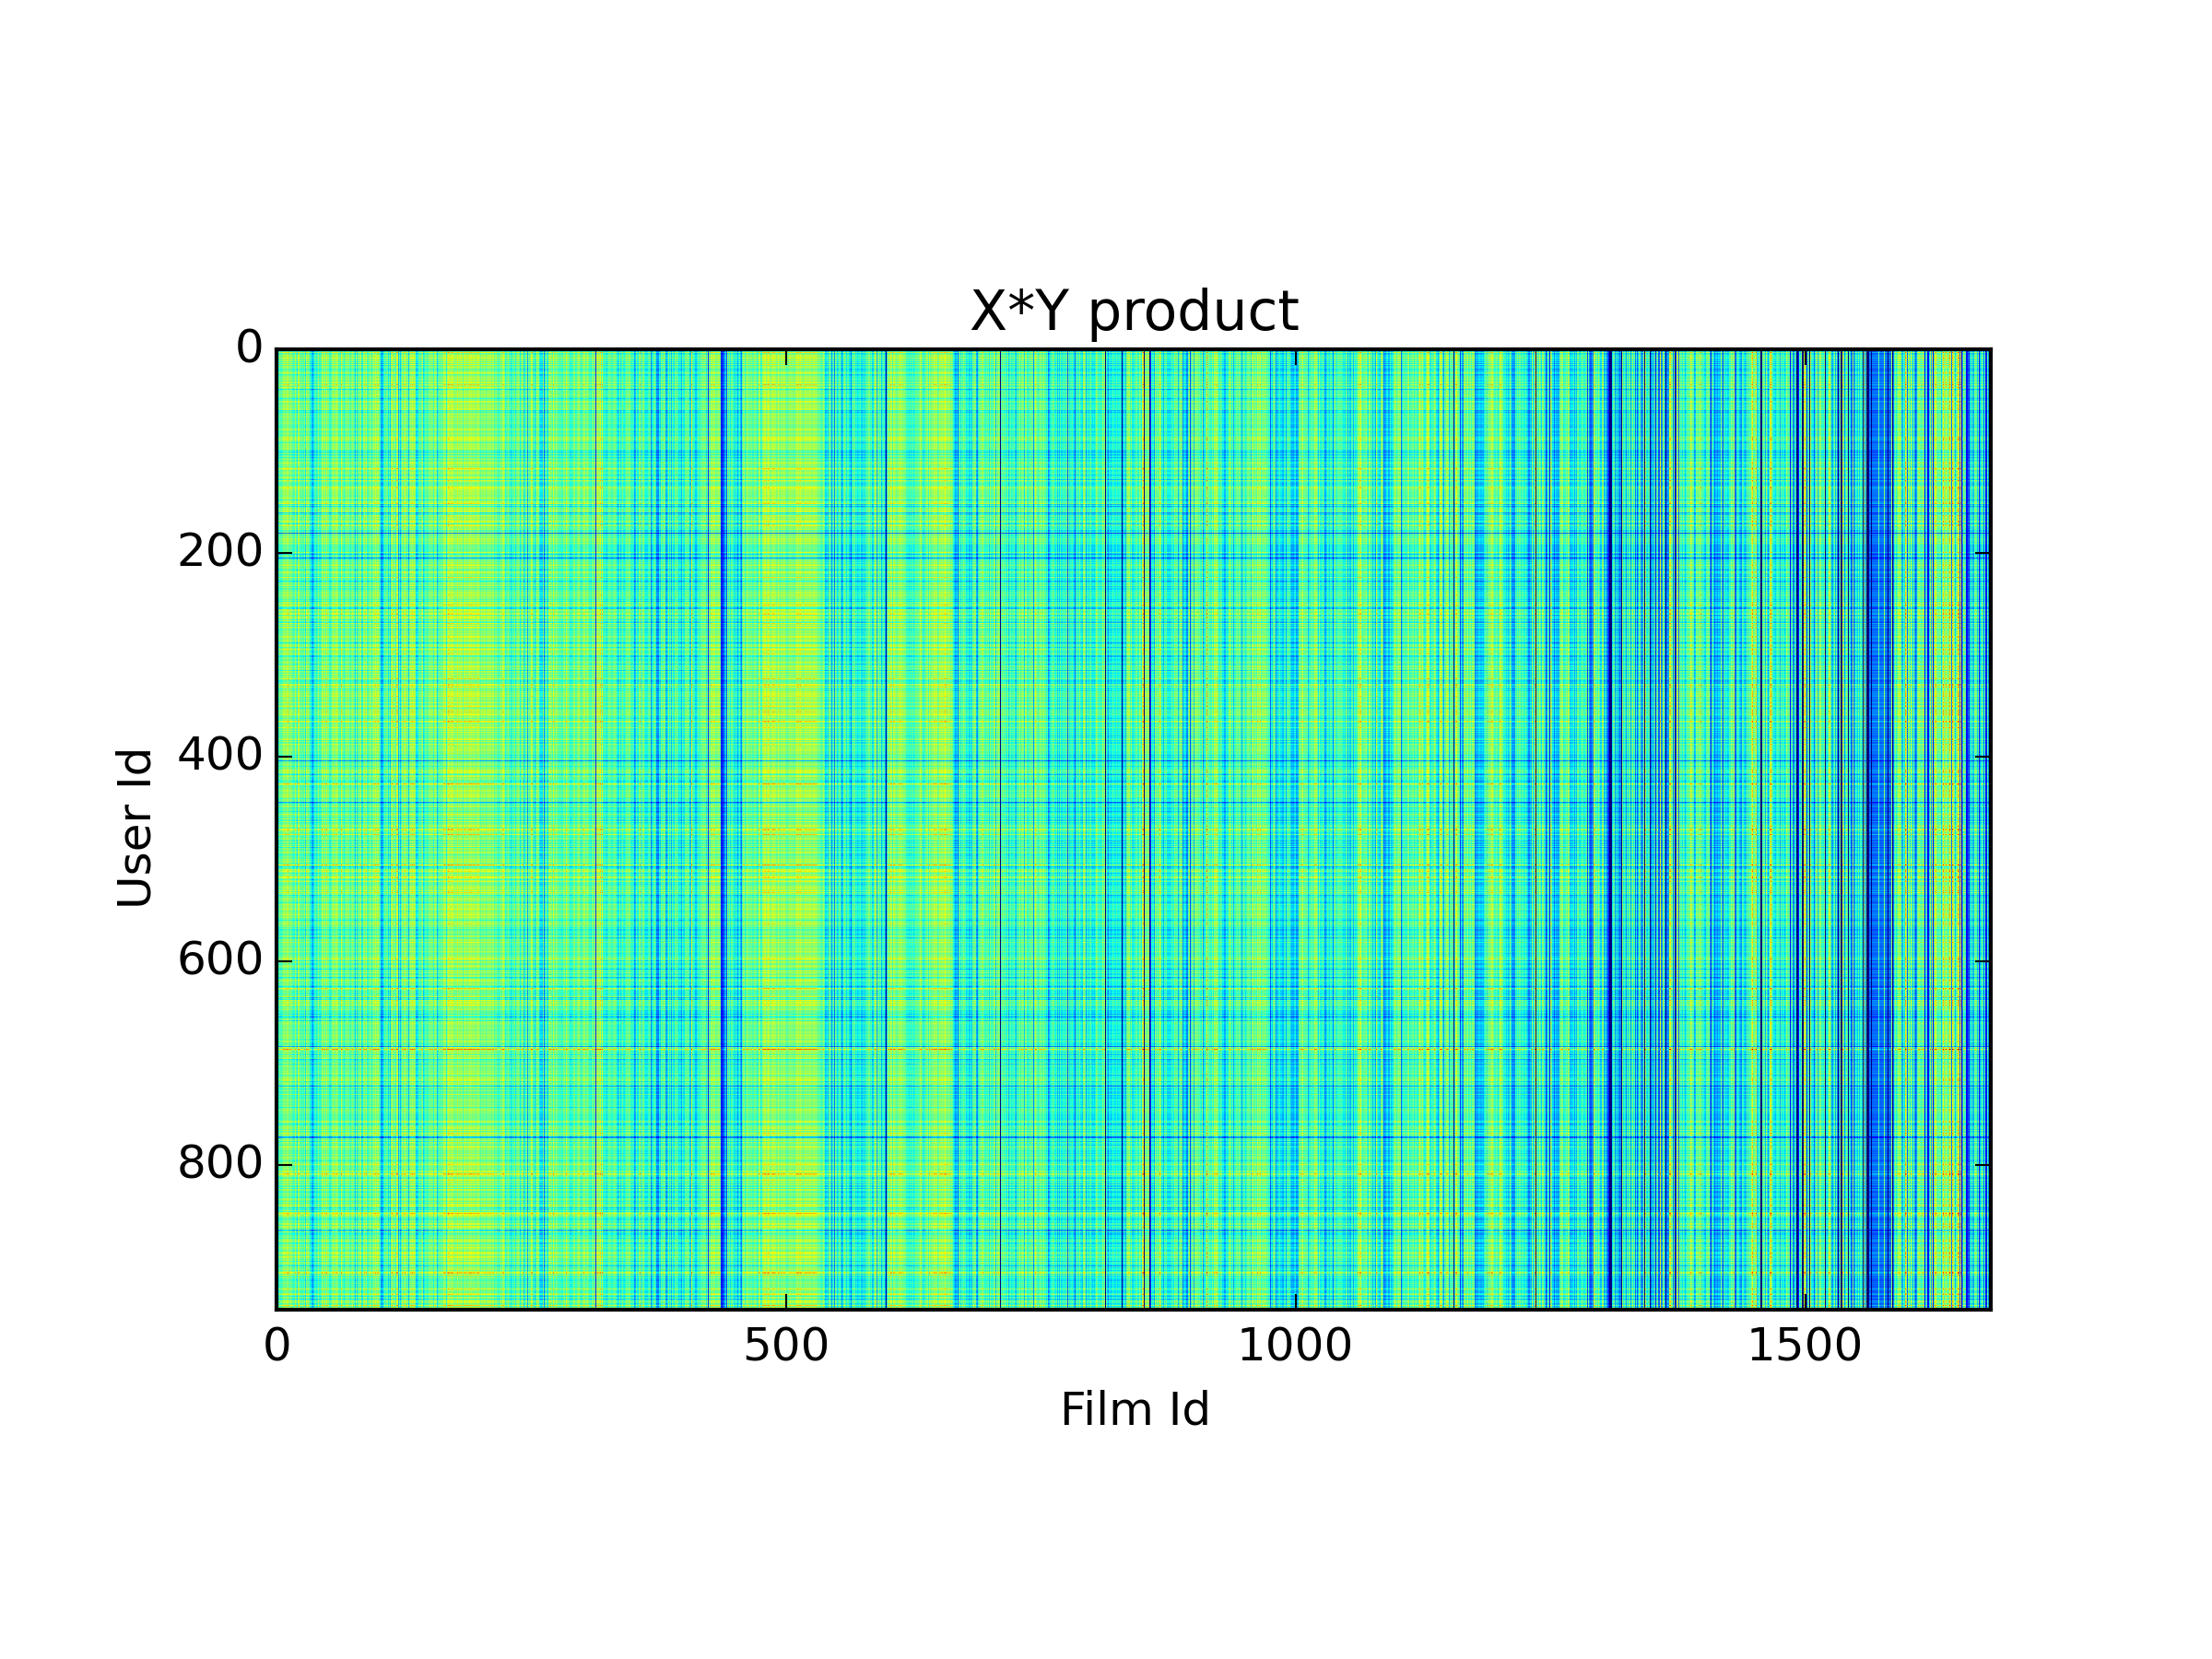
\includegraphics[scale=0.2]{it2-k3-l2.png}}
&
\subfloat[X*Y à la $3^e$ itération]{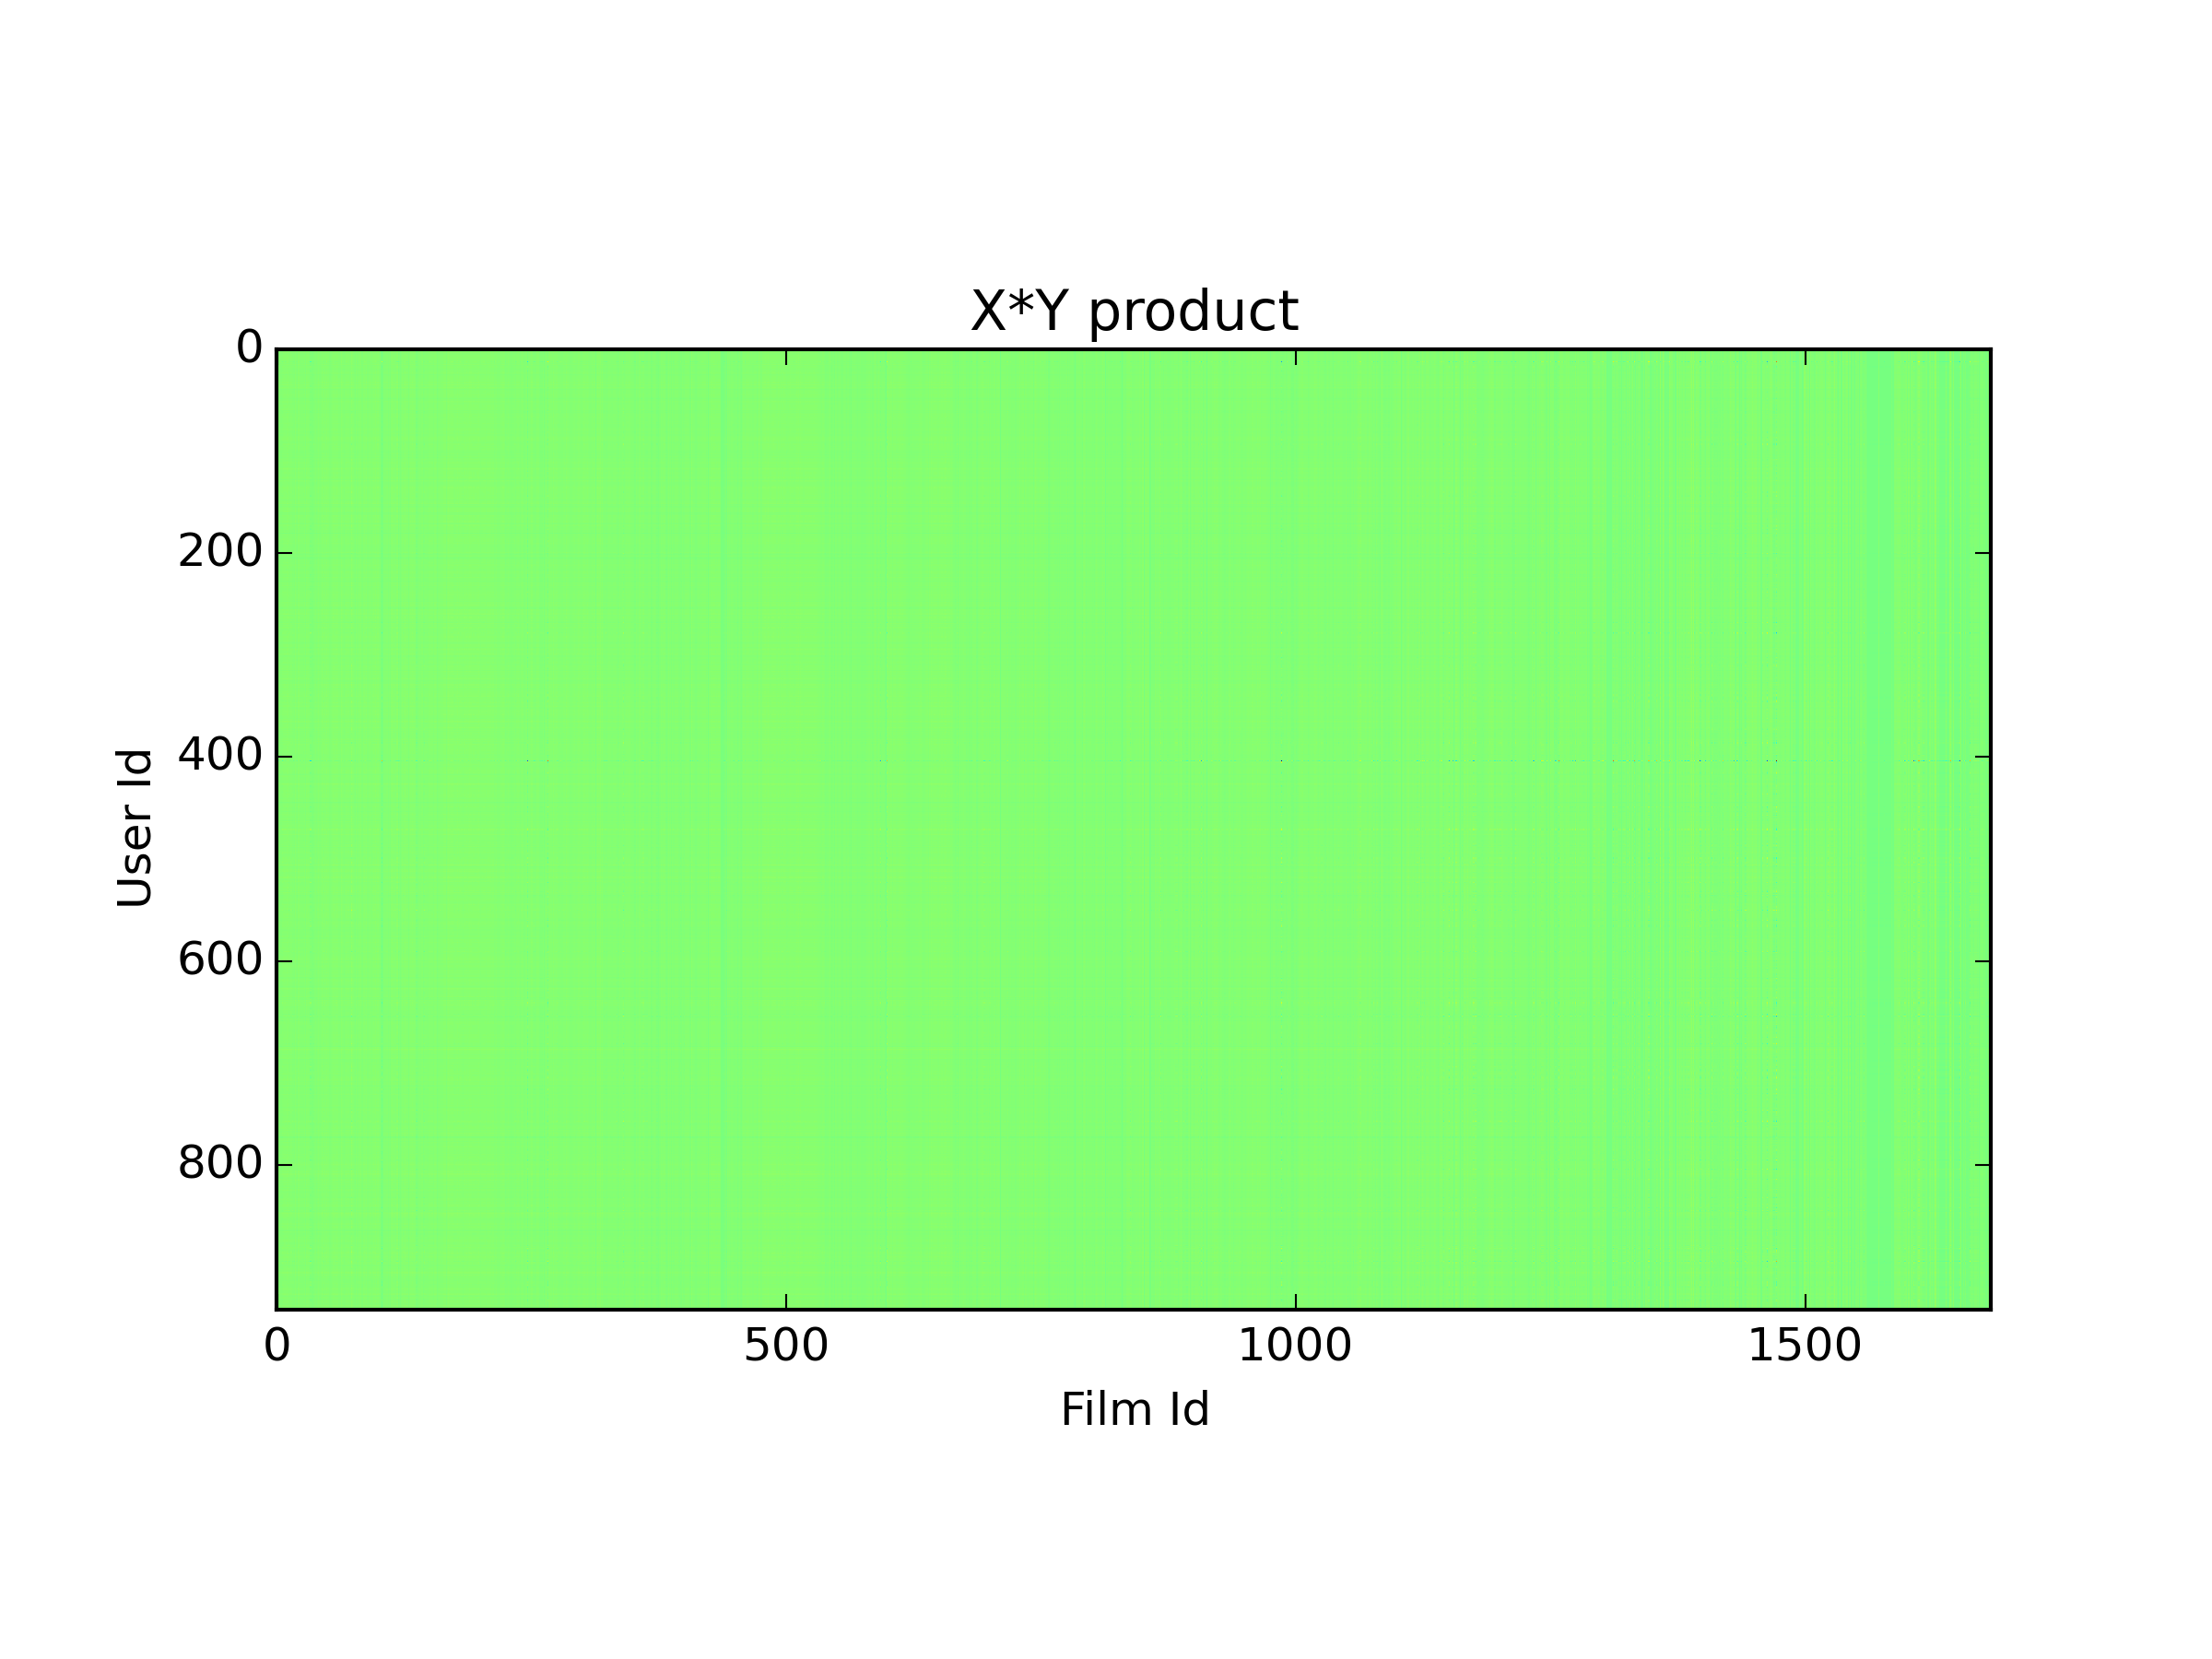
\includegraphics[scale=0.2]{it3-k3-l2.png}}
&
\subfloat[X*Y à la $10^e$ itération]{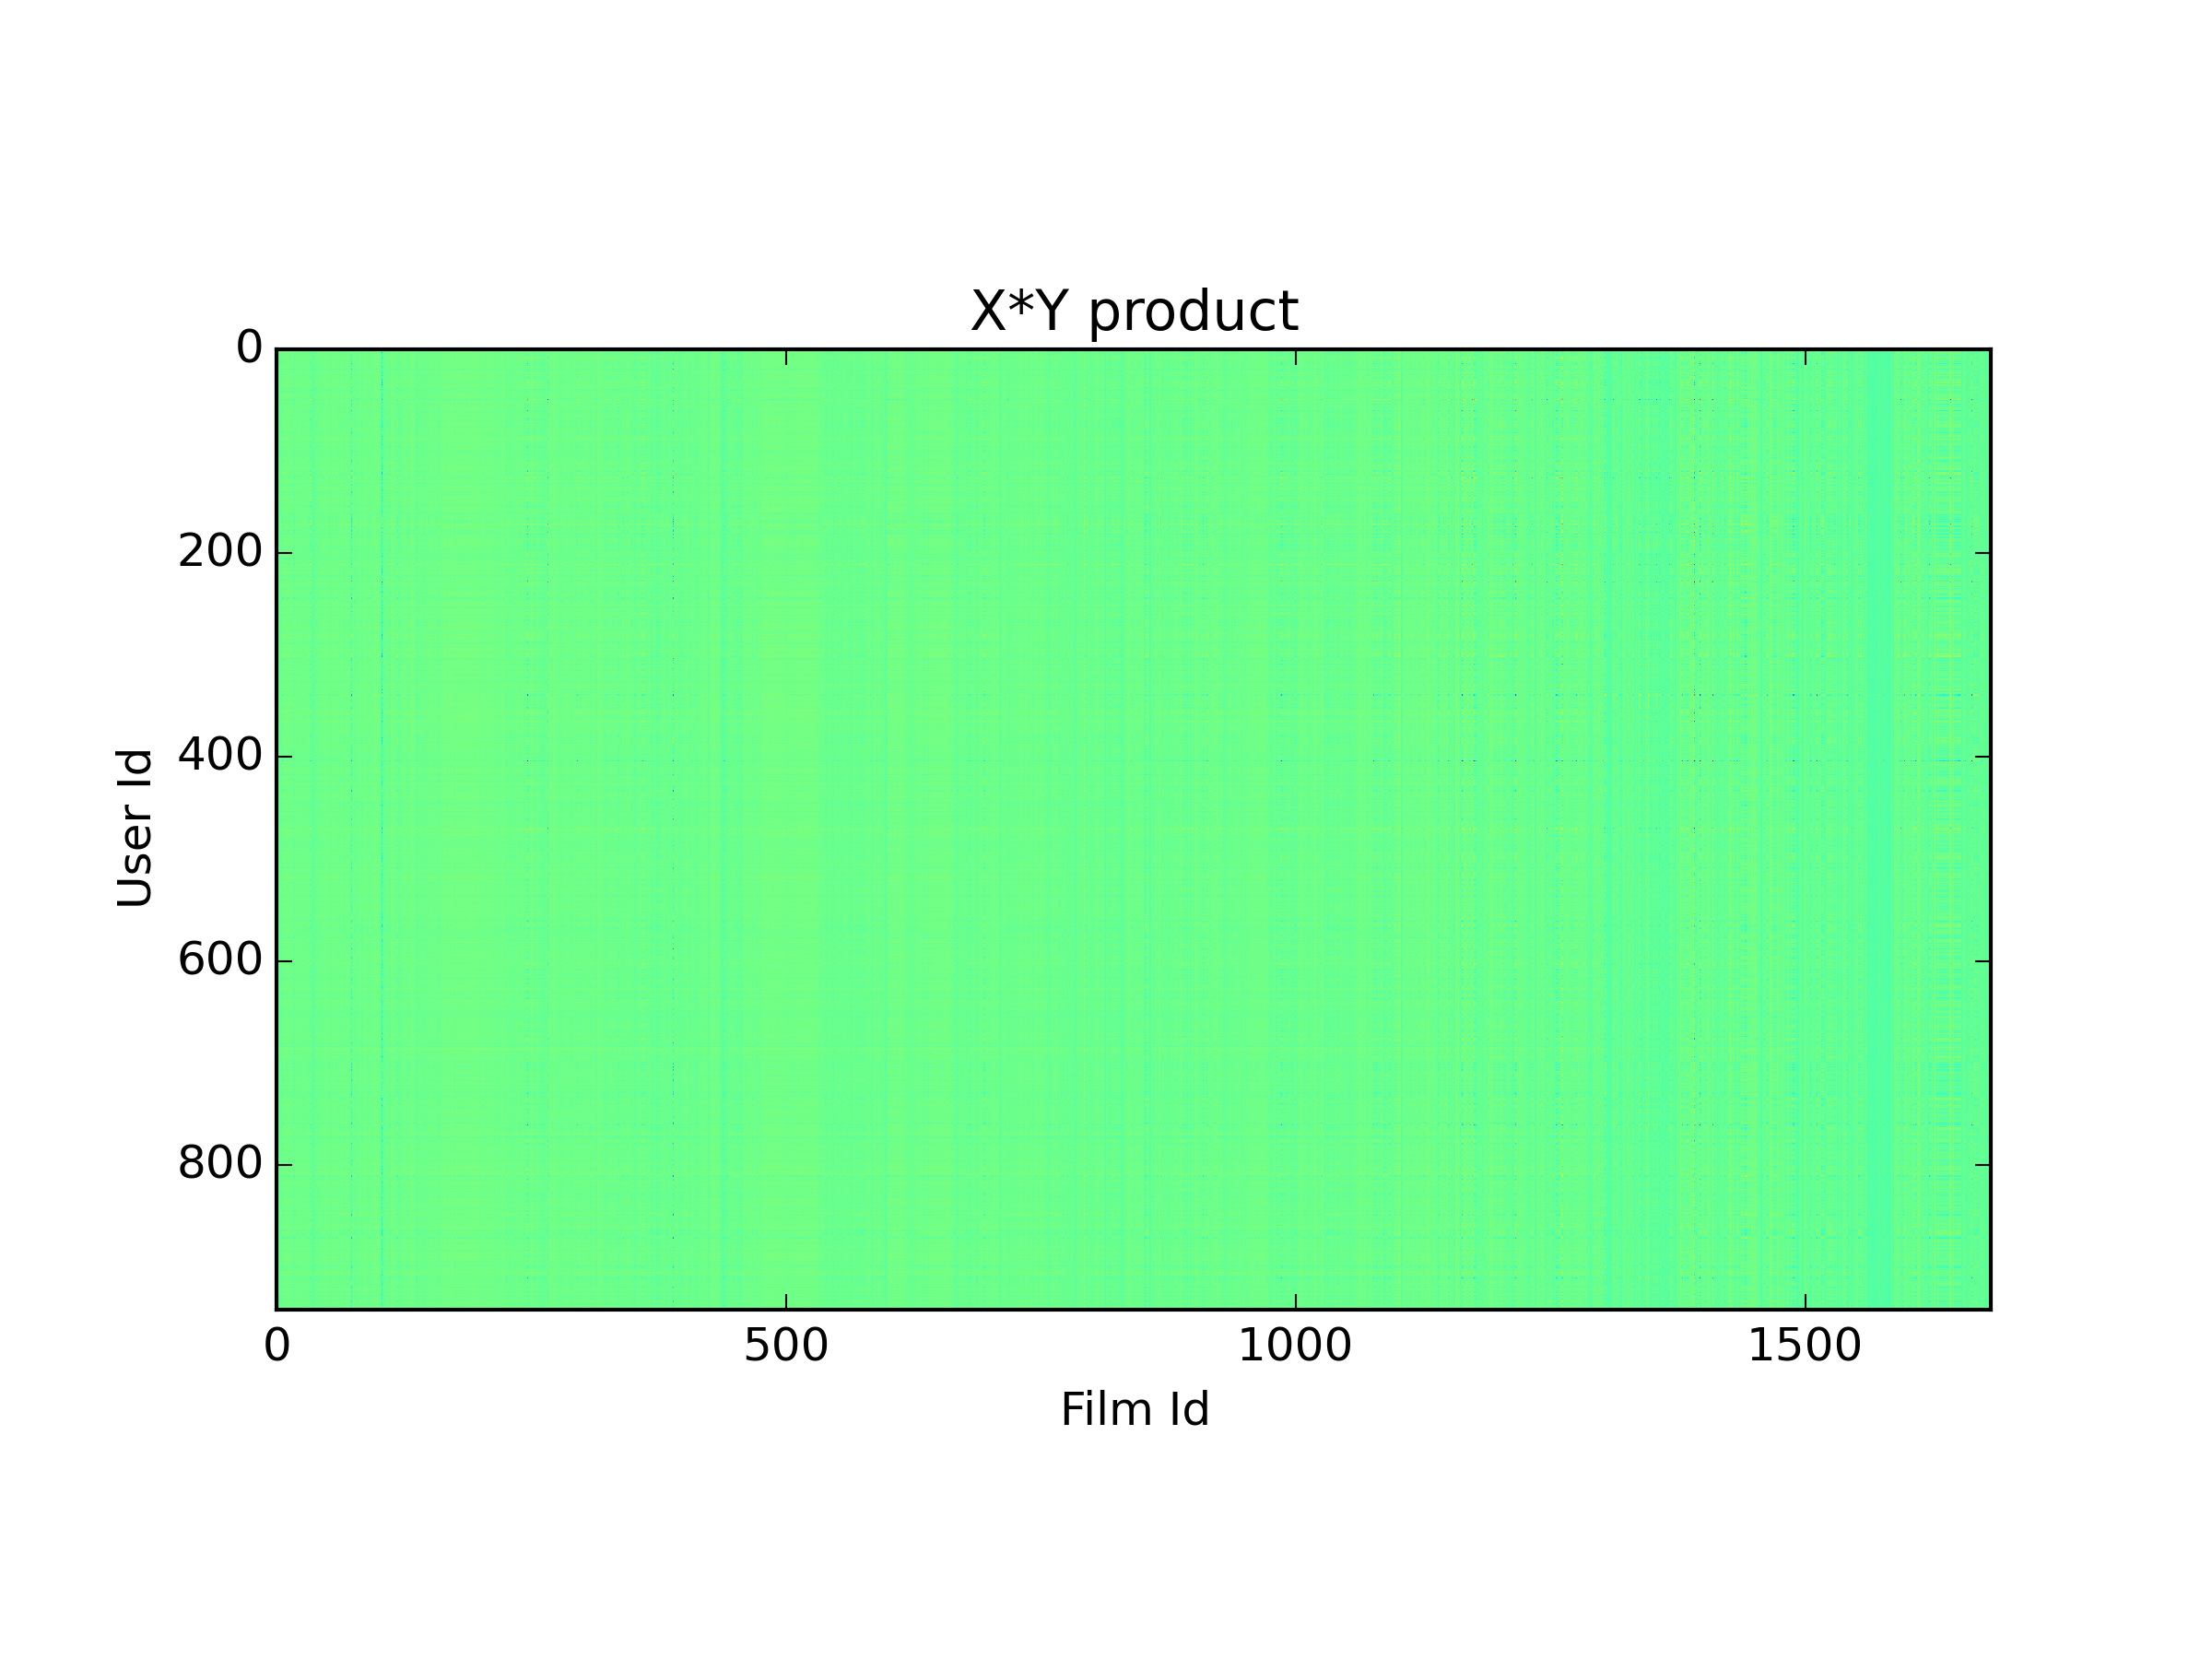
\includegraphics[scale=0.2]{it10-k3-l2.png}}
\end{tabular}
\caption{Pour k=3, $\lambda$=0.02}
\end{table}

\begin{table}[h]
\begin{tabular}{cccc}
\subfloat[X*Y à la $1^{ere}$ itération]{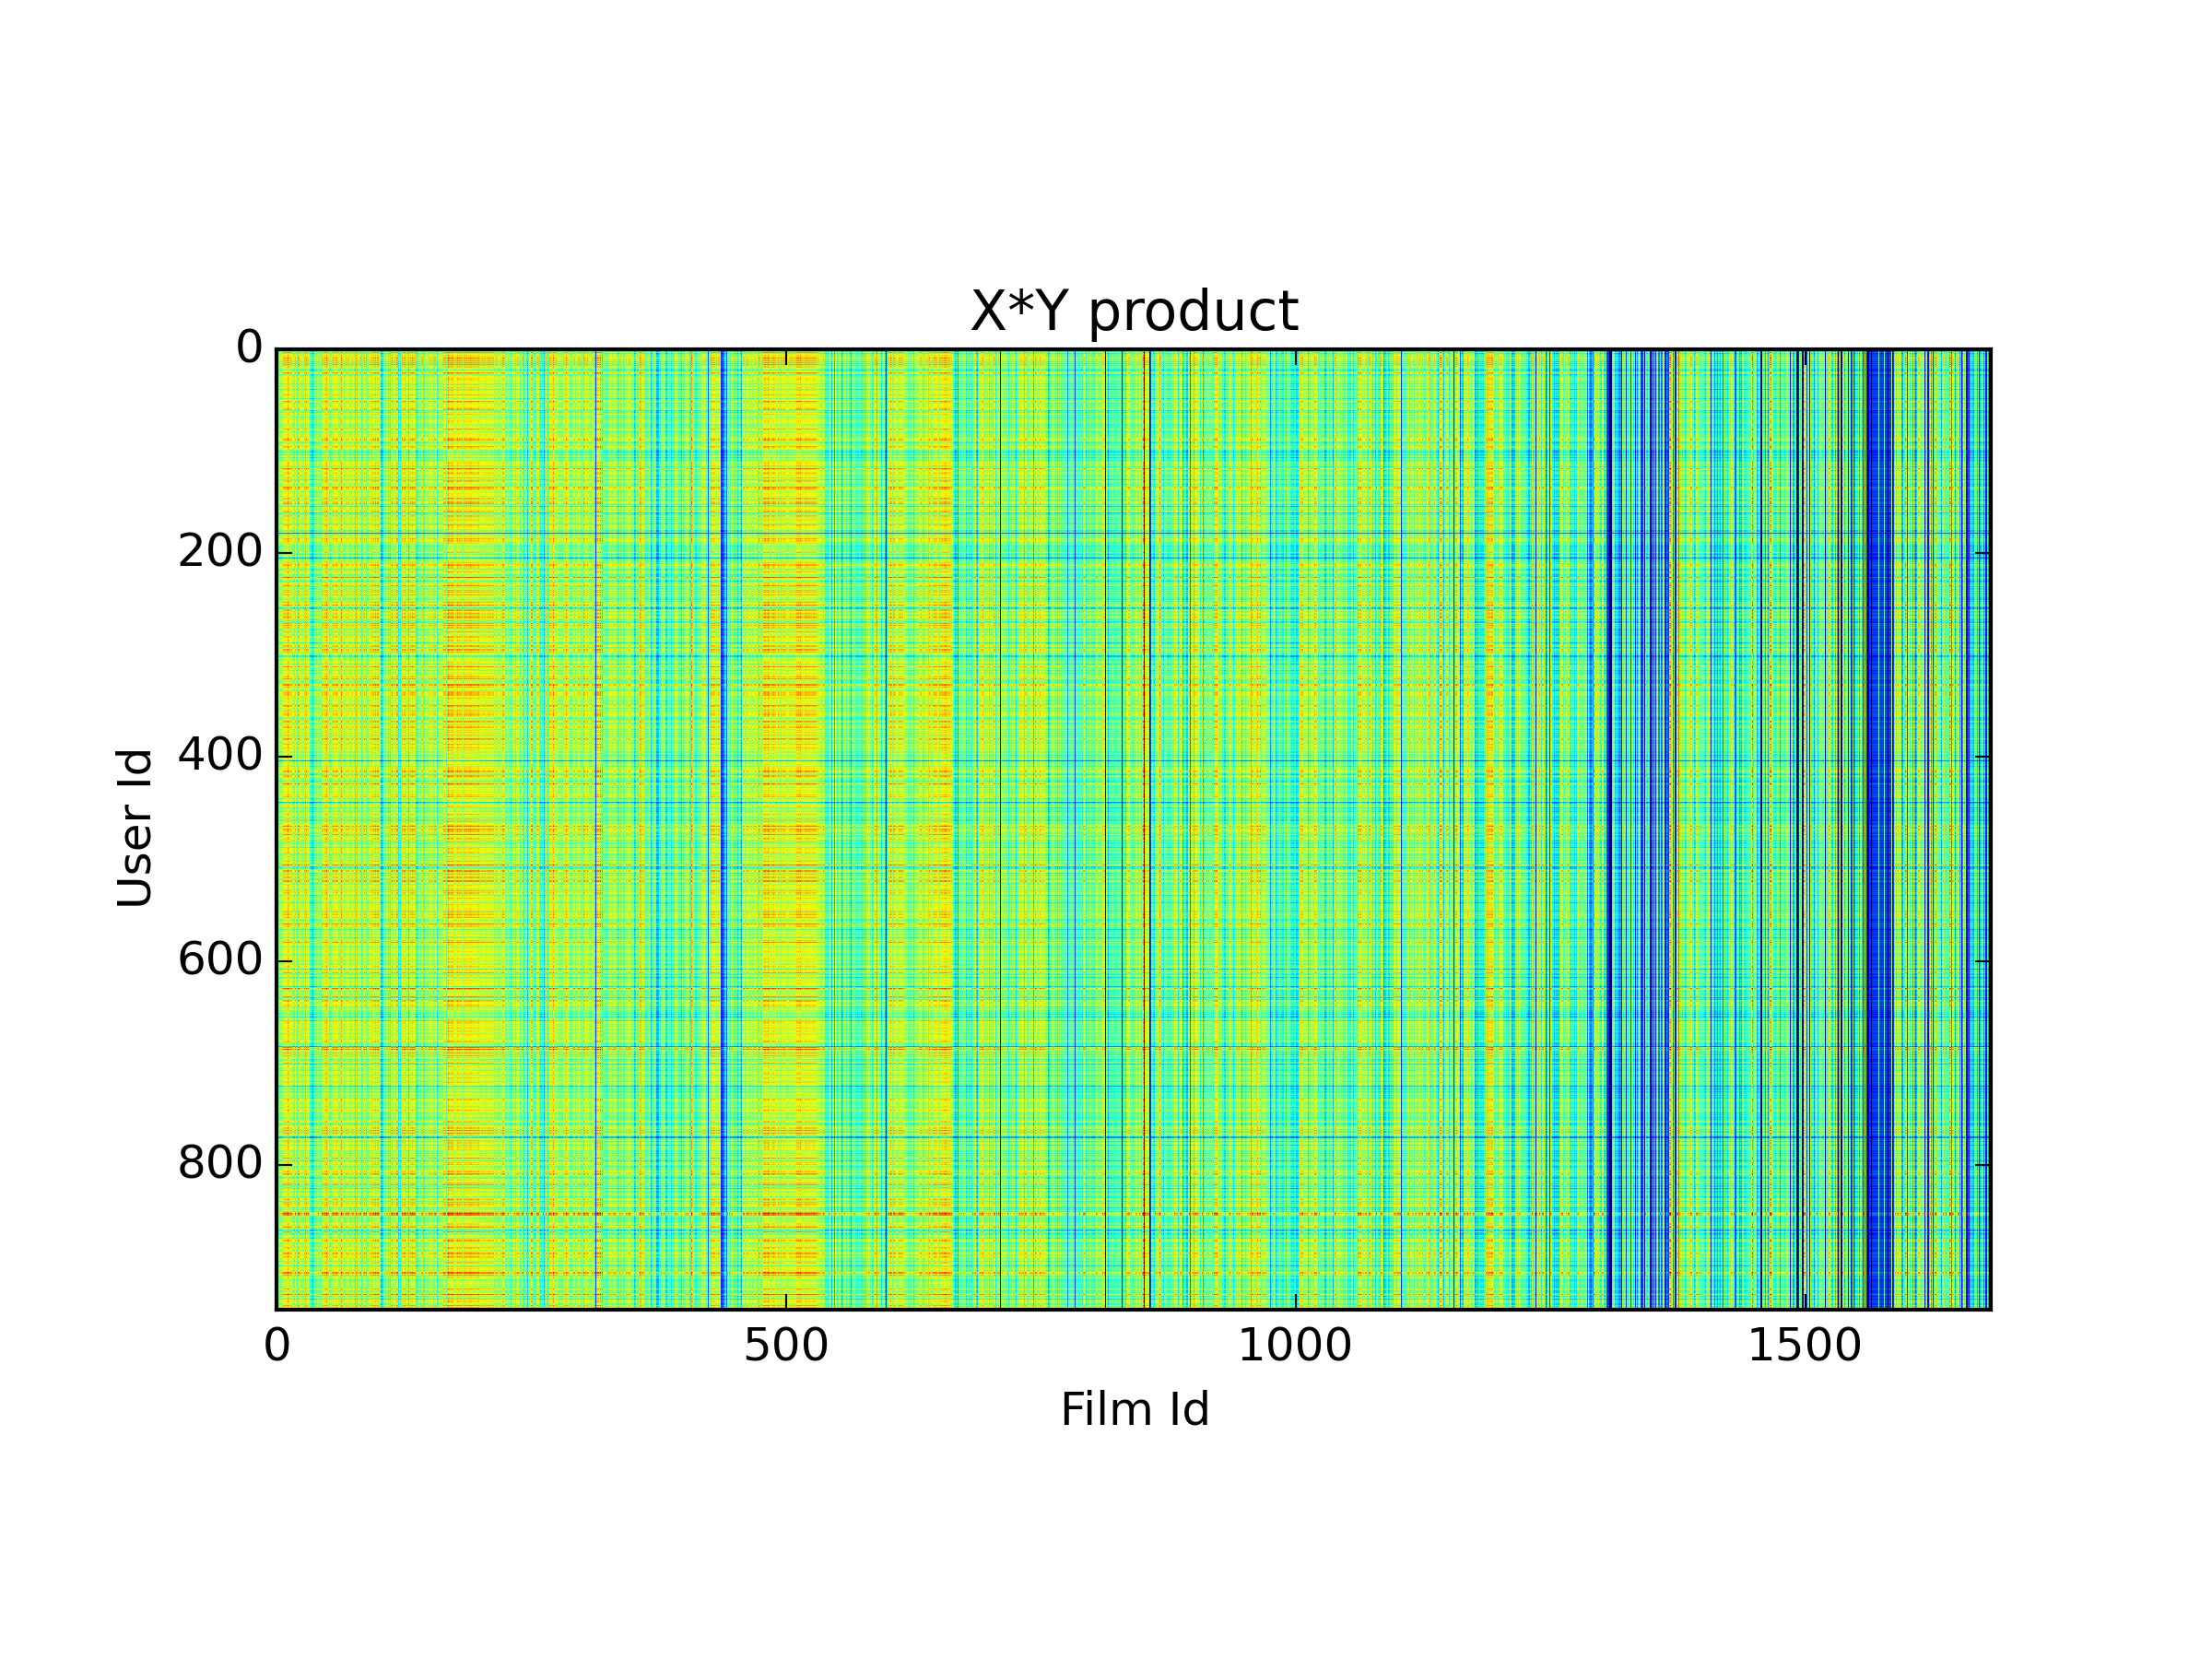
\includegraphics[scale=0.2]{it1-k3-l80.png}}
&
\subfloat[X*Y à la $2^e$ itération]{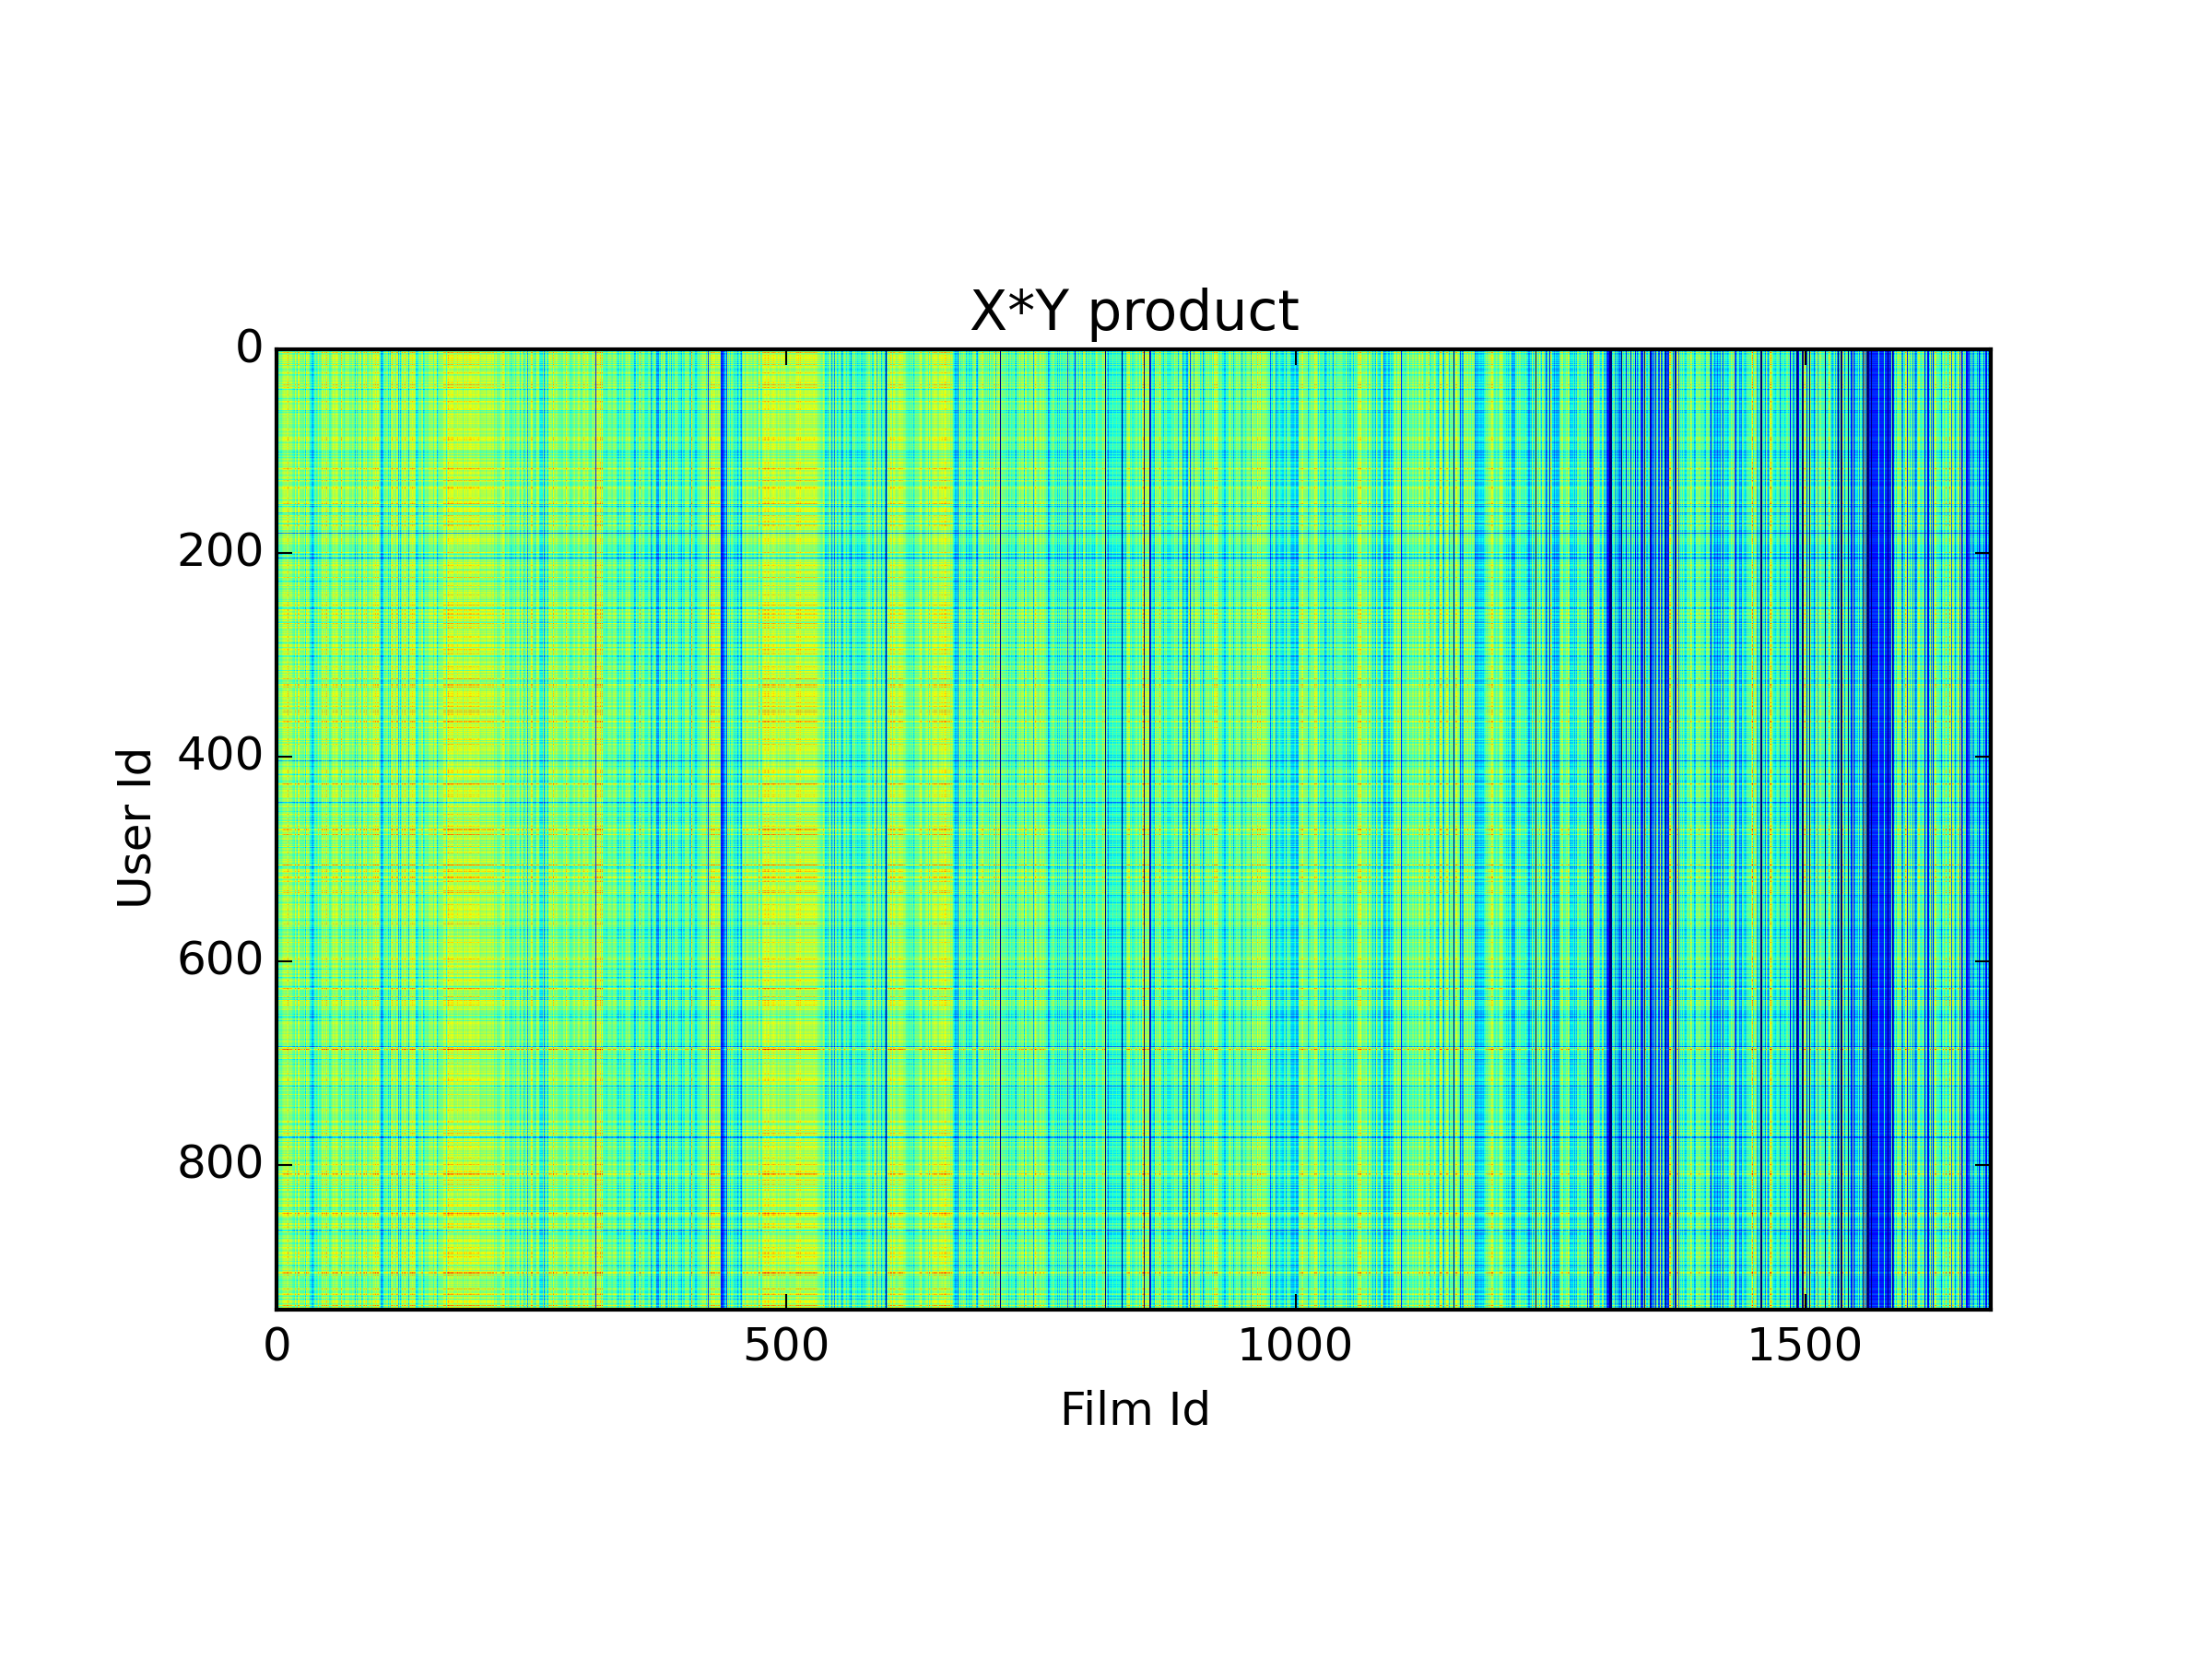
\includegraphics[scale=0.2]{it2-k3-l80.png}}
&
\subfloat[X*Y à la $10^e$ itération]{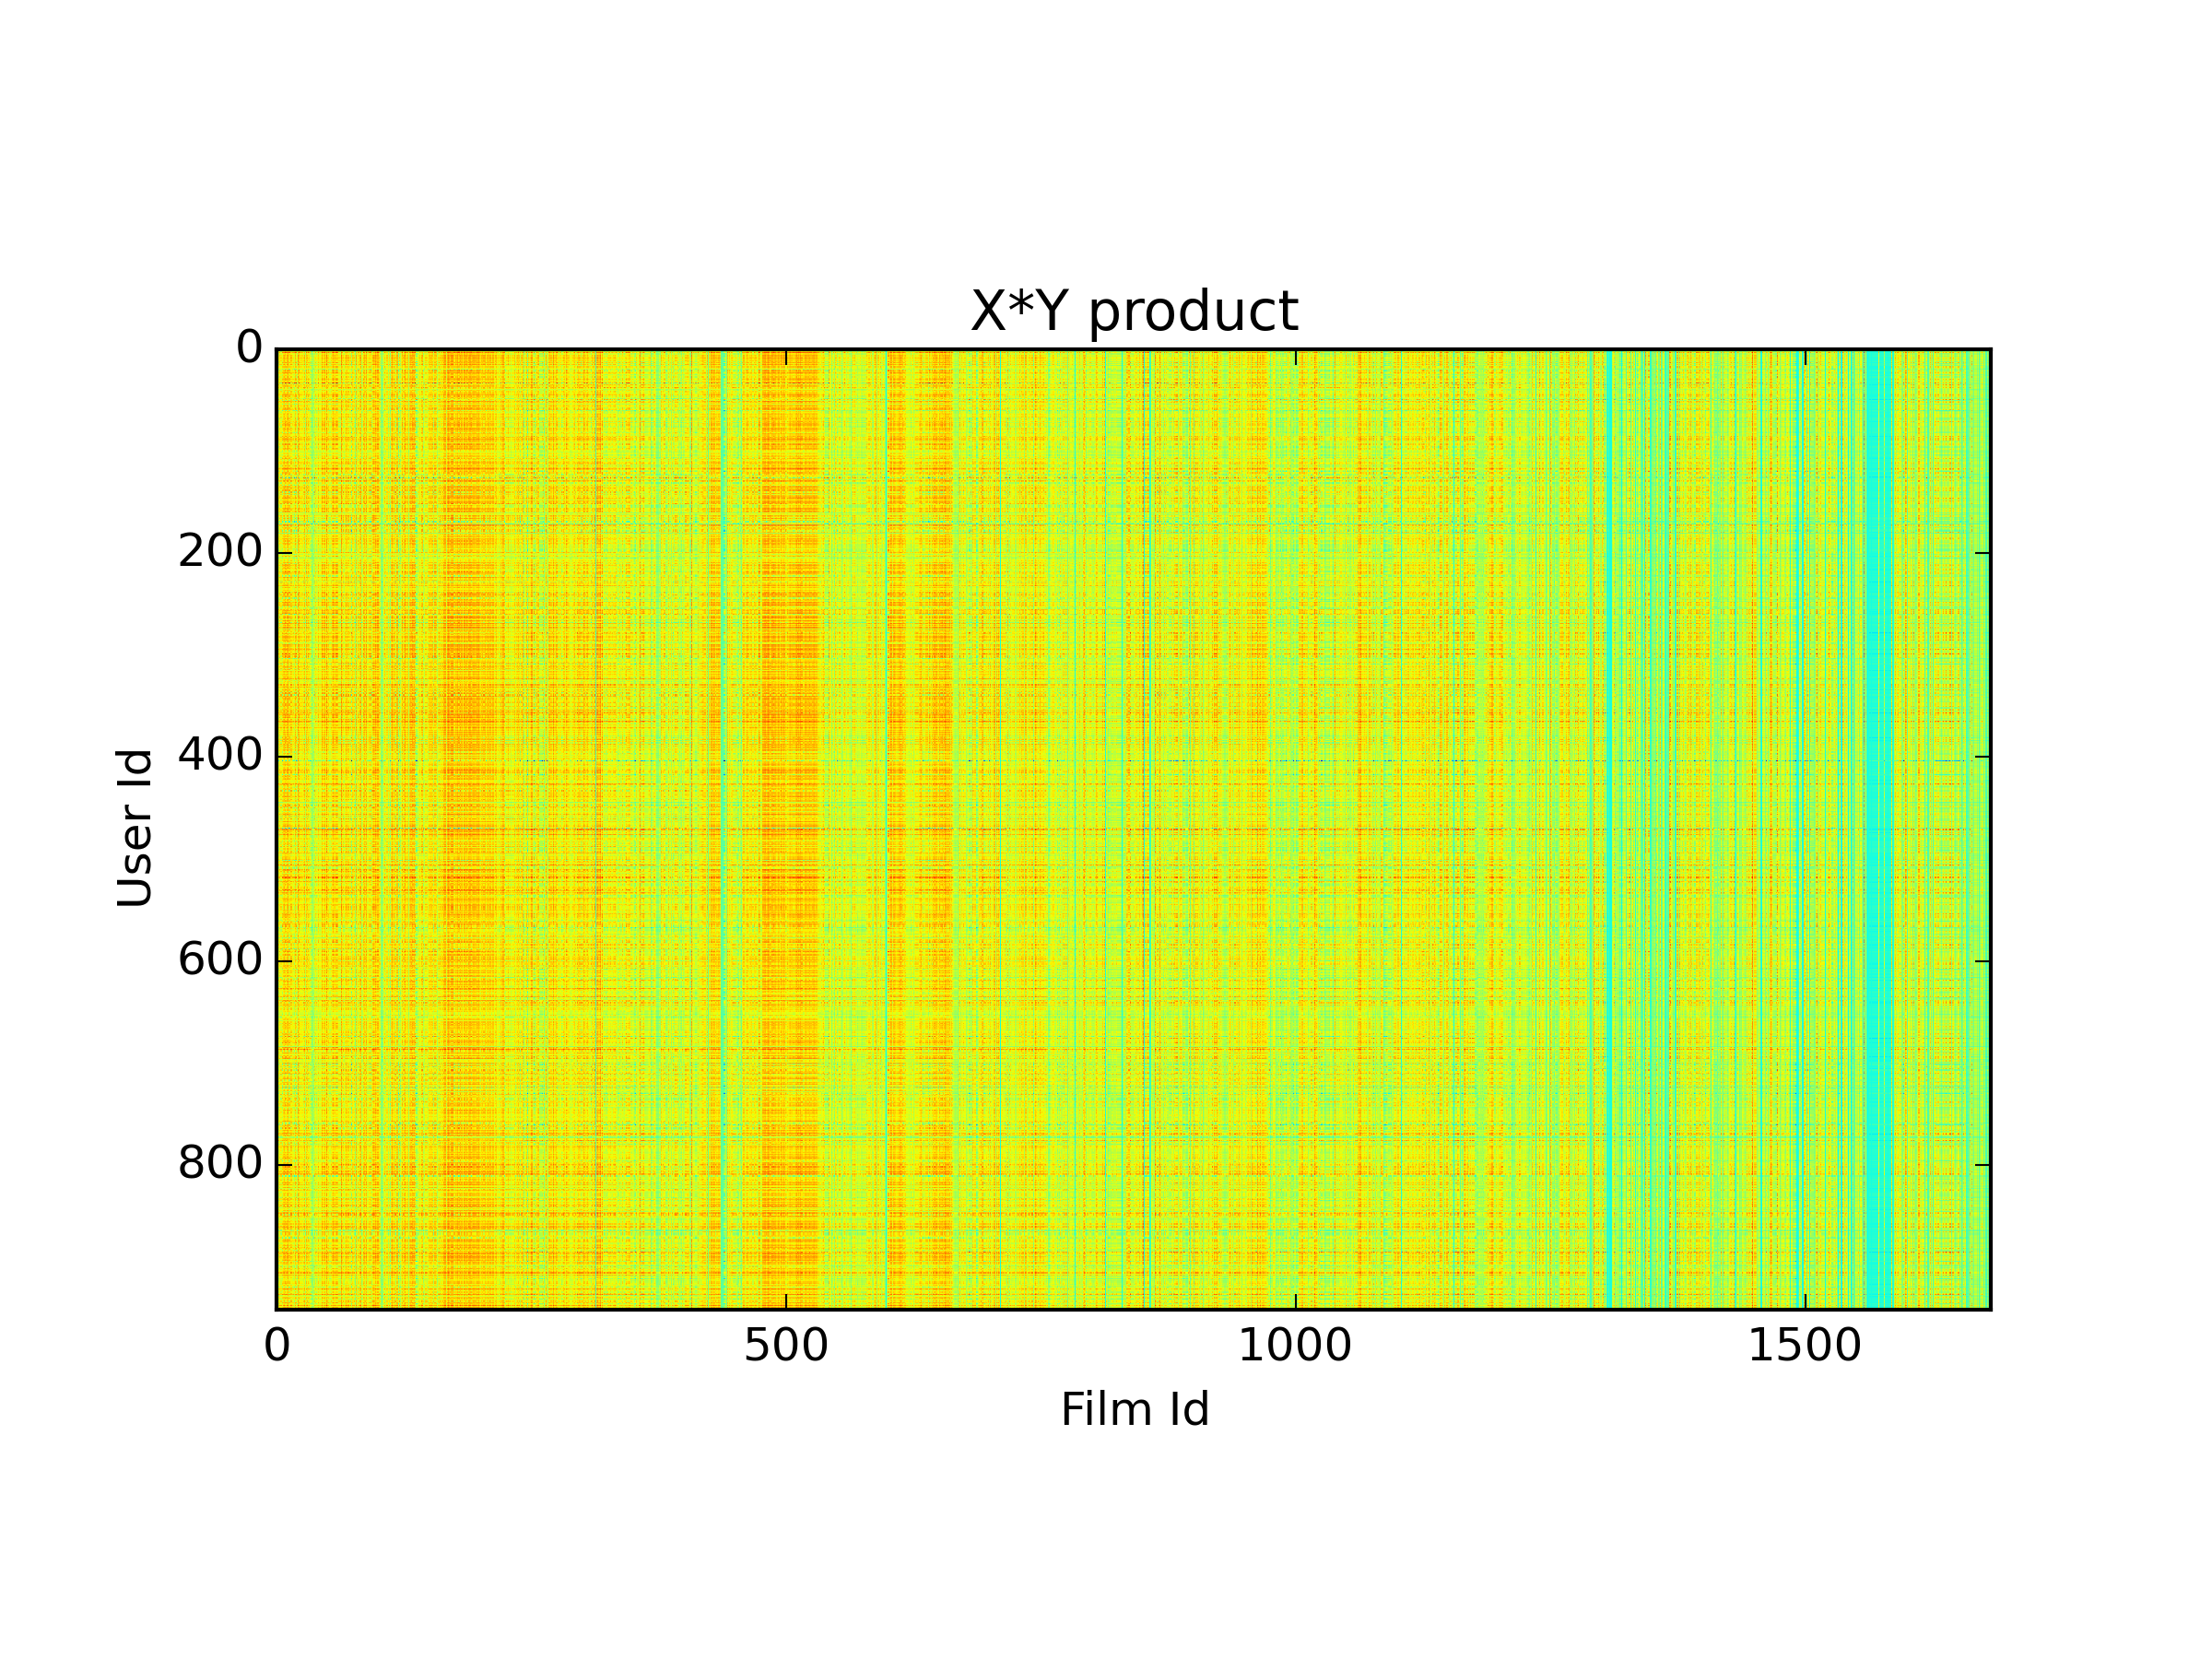
\includegraphics[scale=0.2]{it10-k3-l80.png}}
&
\subfloat[X*Y à la $50^e$ itération]{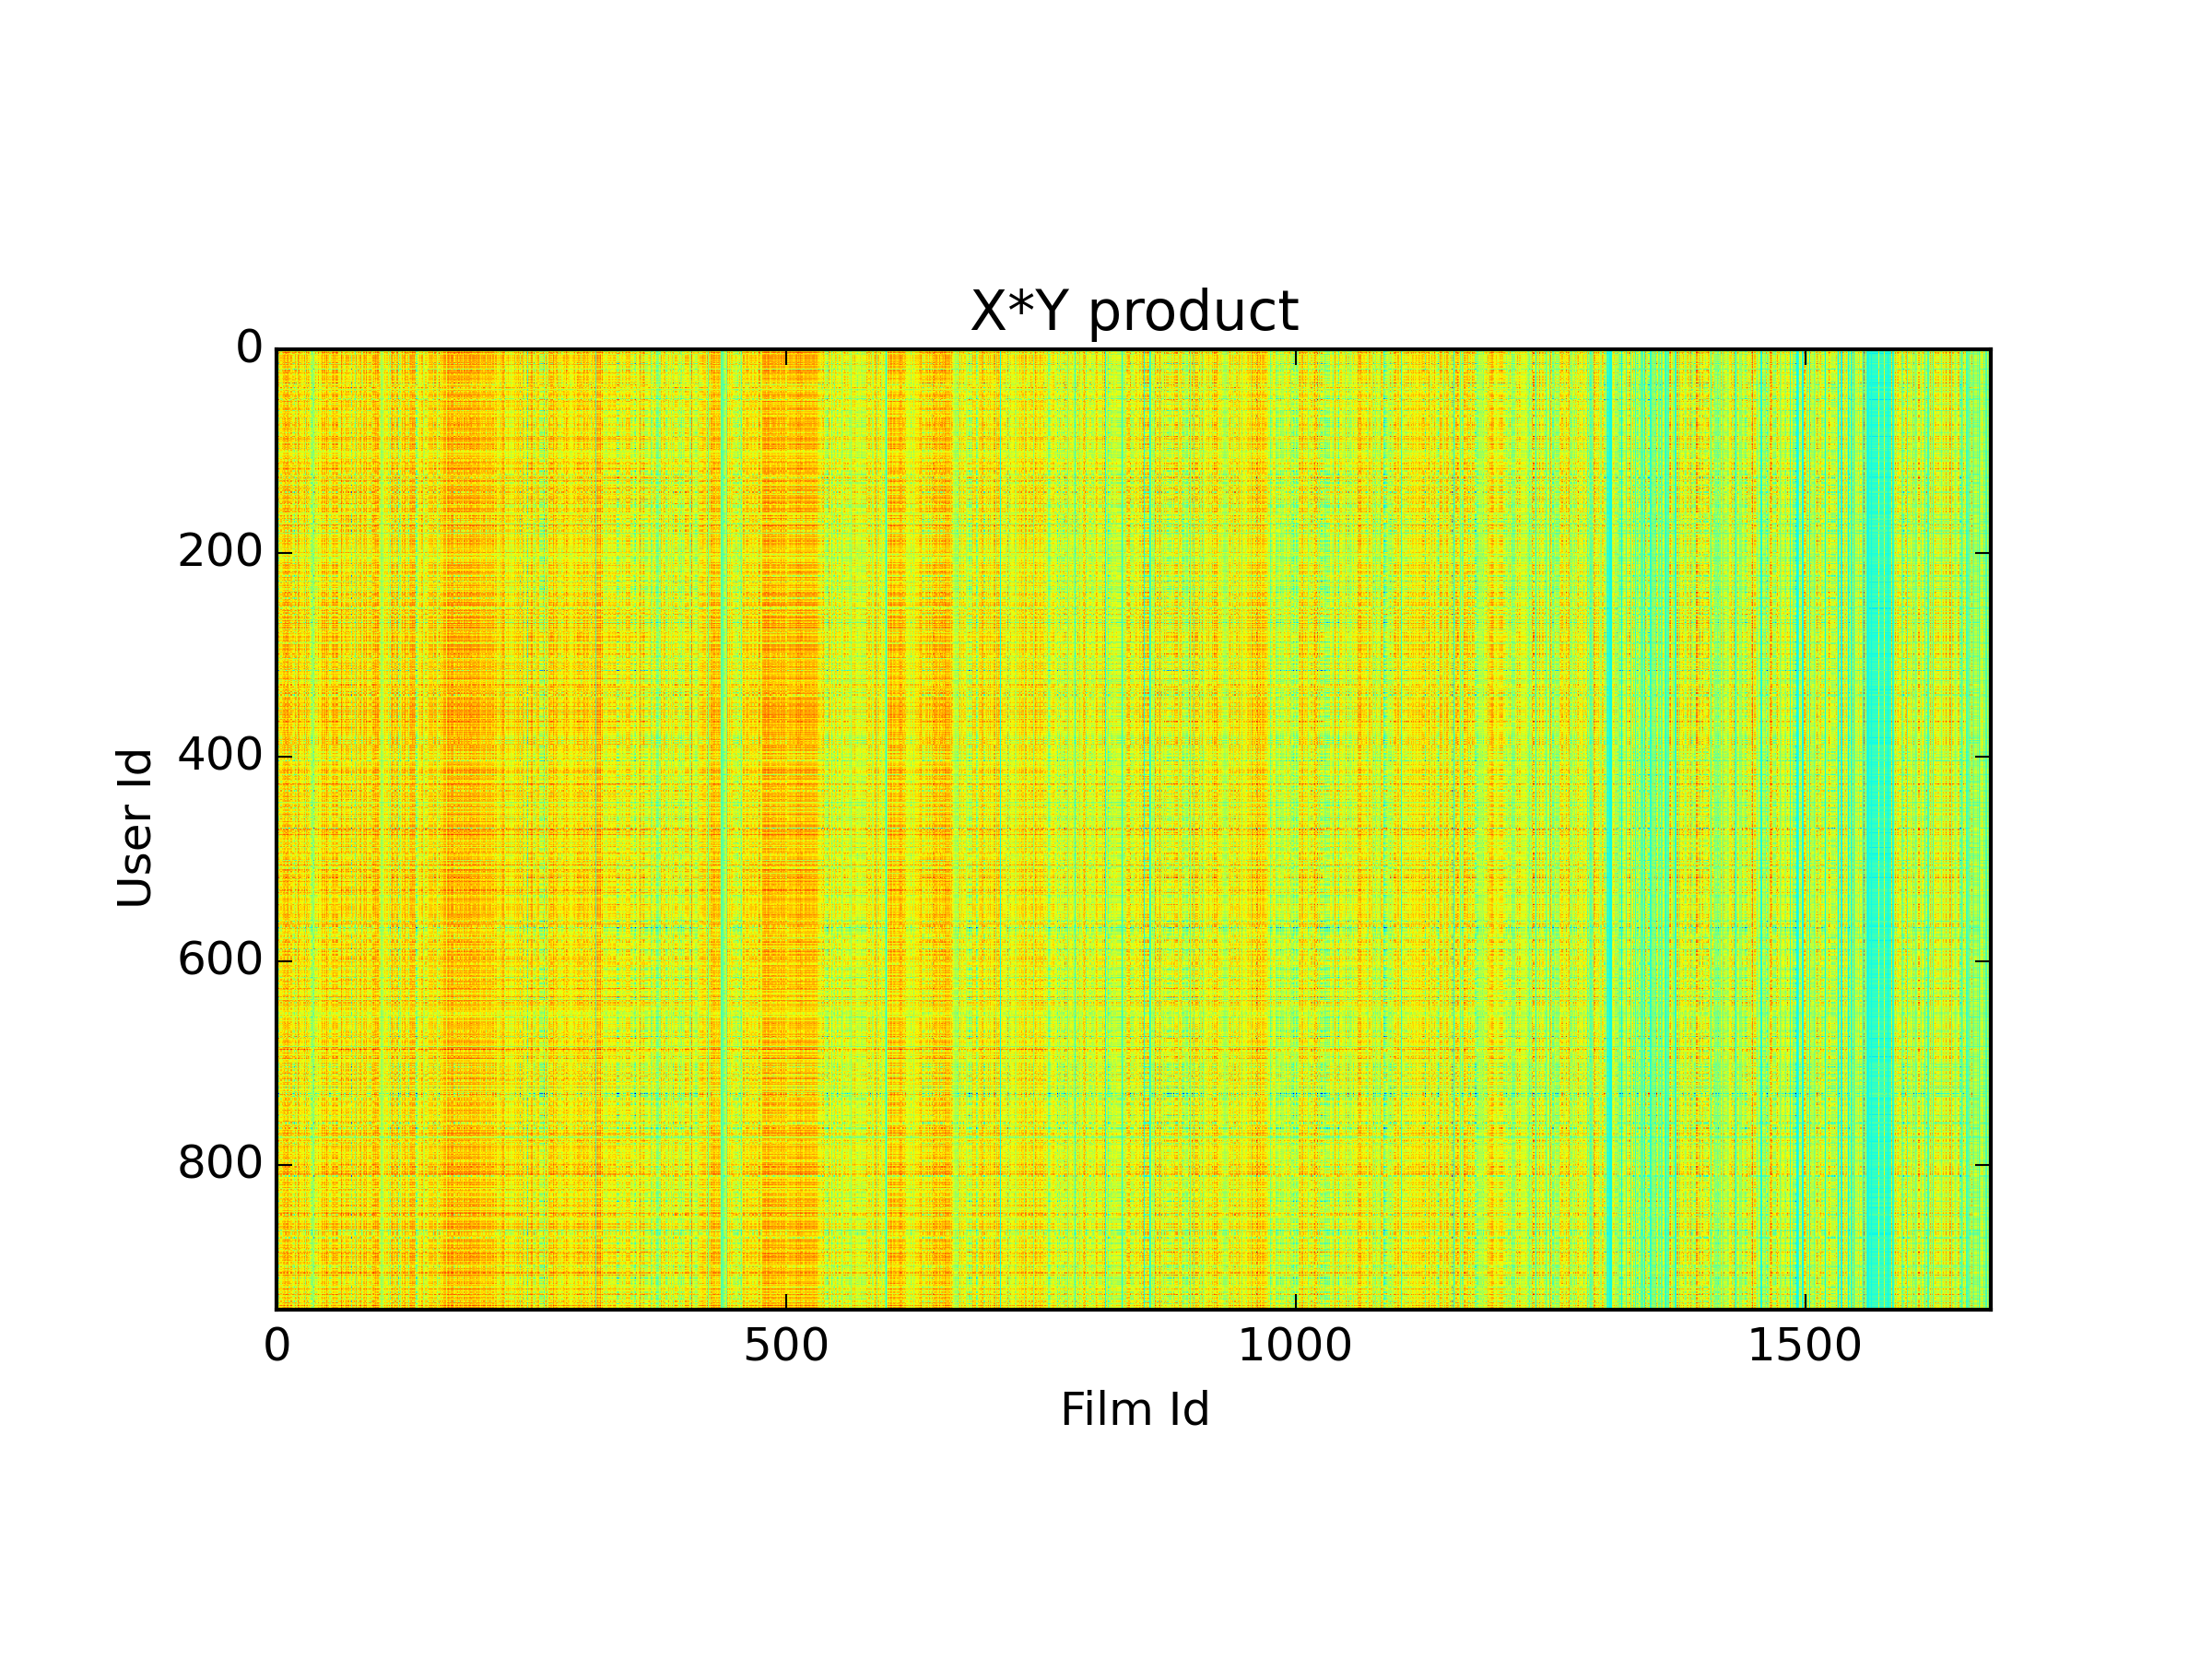
\includegraphics[scale=0.2]{it35-k3-l80.png}}
\end{tabular}
\caption{Pour k=3, $\lambda$=0.80}
\end{table}
\newpage


\begin{table}[h]
\begin{tabular}{cc}
\subfloat[Pour k=12 ; $\lambda=0.02$]{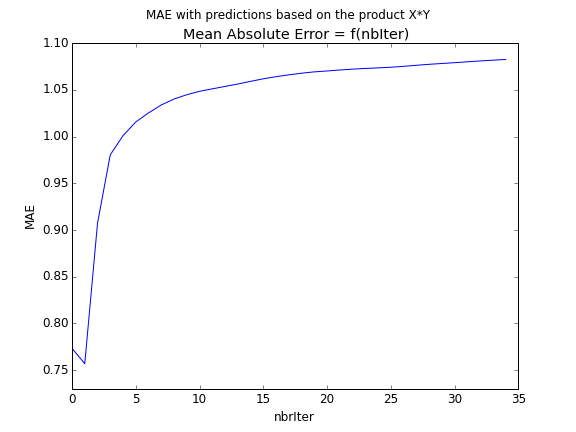
\includegraphics[scale=0.4]{MAE-least-squares-k12-l2.png}}
&
\subfloat[Pour k=12 ; $\lambda=0.80$]{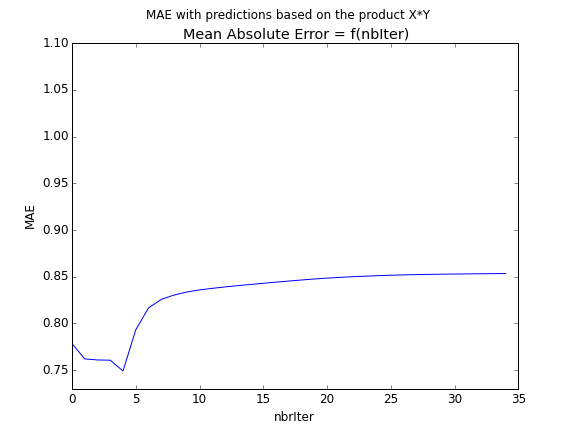
\includegraphics[scale=0.4]{MAE-least-squares-k12-l80.png}}
\end{tabular}
\end{table}

\begin{table}[h]
\begin{tabular}{cccc}
\subfloat[X*Y à la $1^{ere}$ itération]{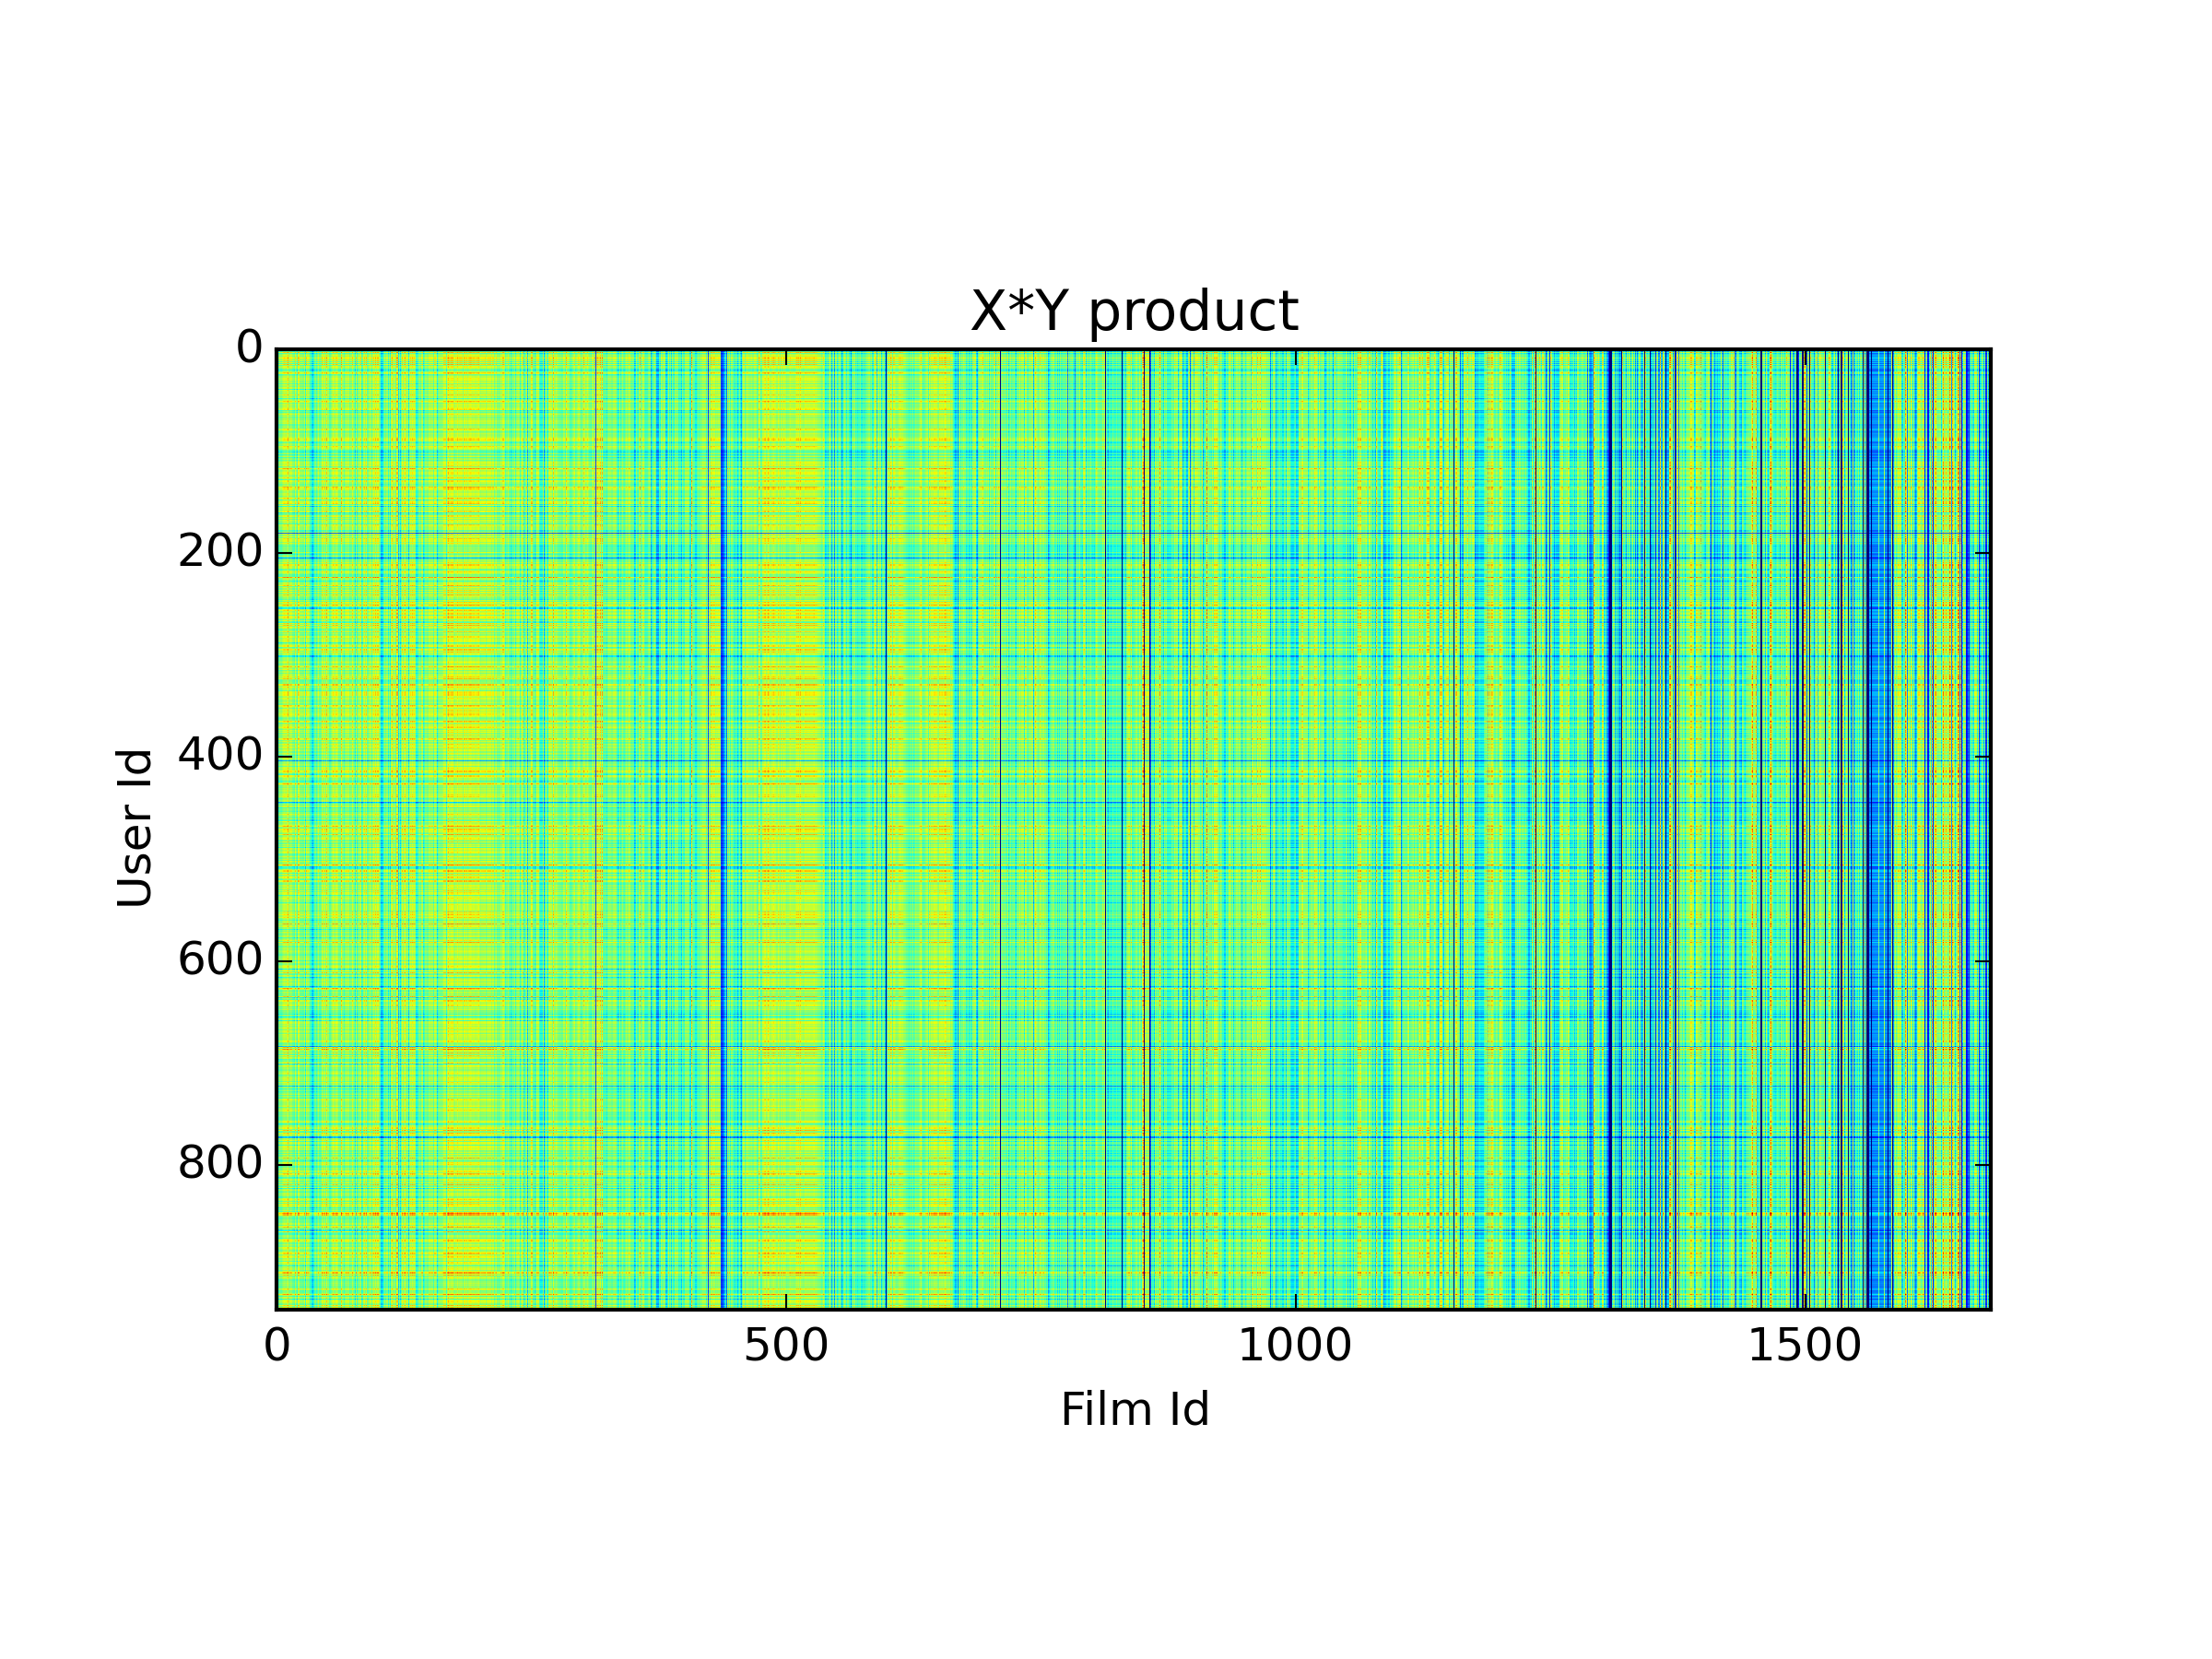
\includegraphics[scale=0.2]{it1-k12-l2.png}}
&
\subfloat[X*Y à la $2^e$ itération \textit{(meilleure MAE)}]{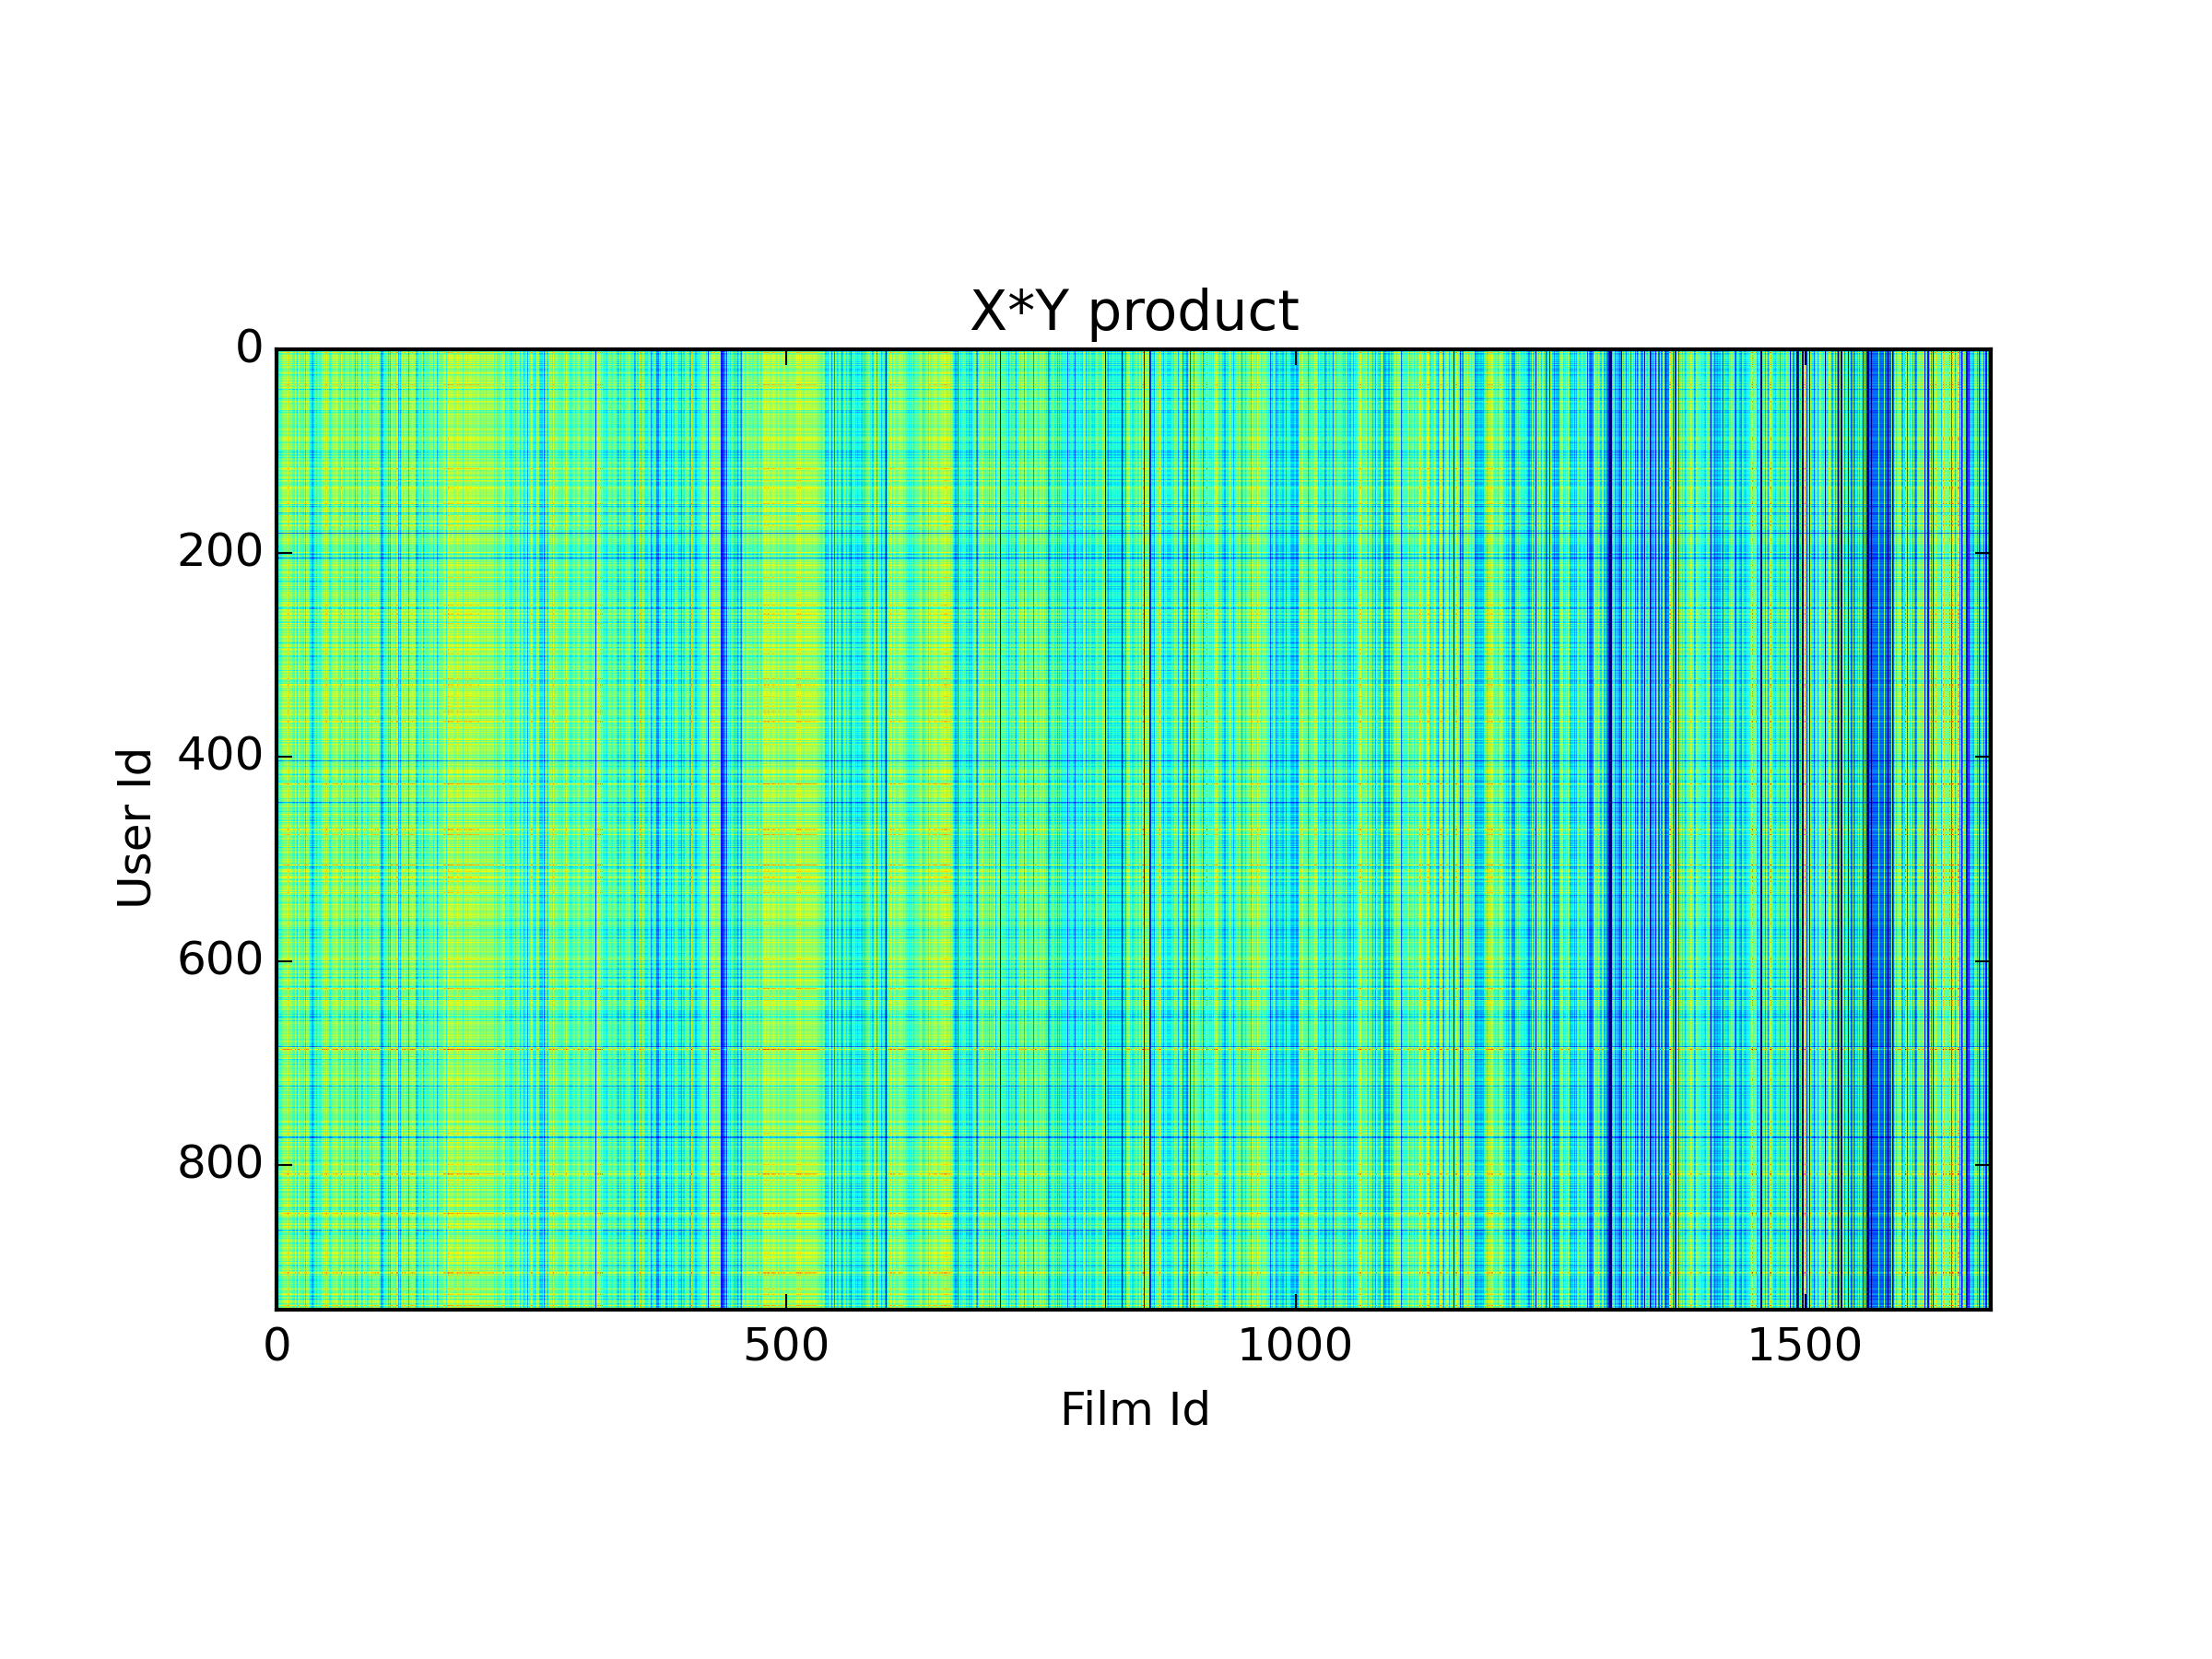
\includegraphics[scale=0.2]{it2-k12-l2.png}}
&
\subfloat[X*Y à la $3^e$ itération]{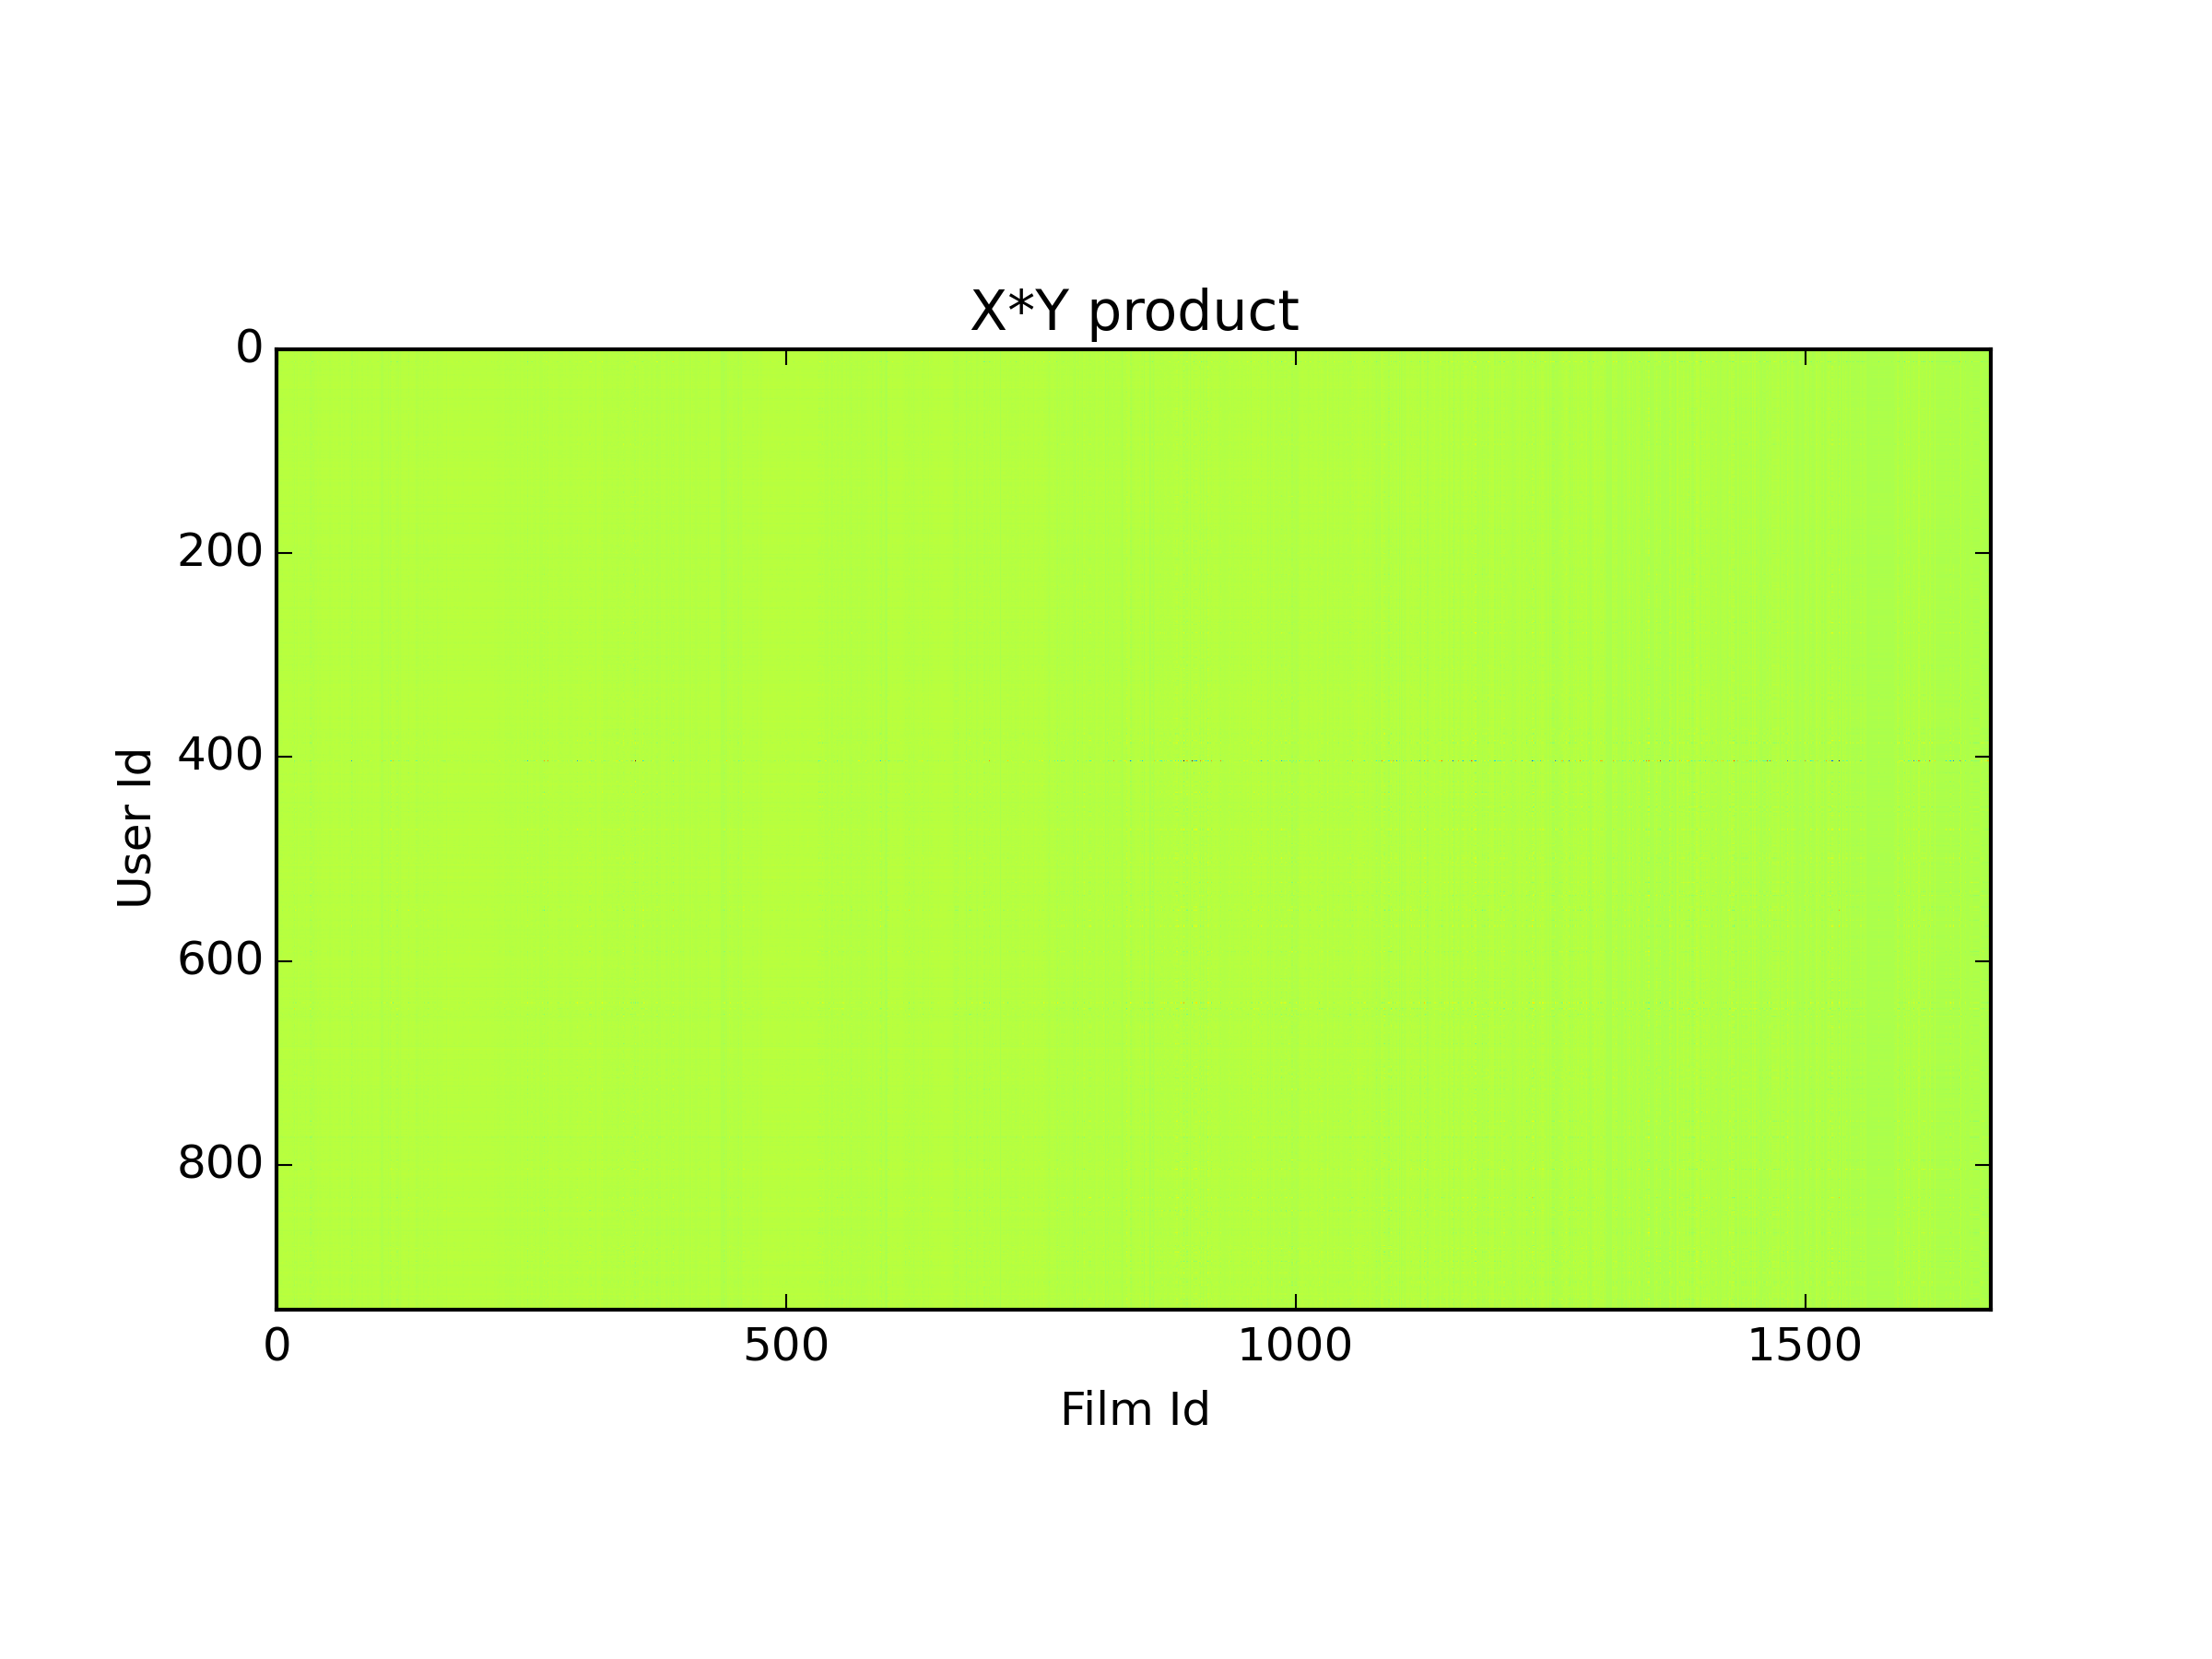
\includegraphics[scale=0.2]{it3-k12-l2.png}}
&
\subfloat[X*Y à la $10^e$ itération]{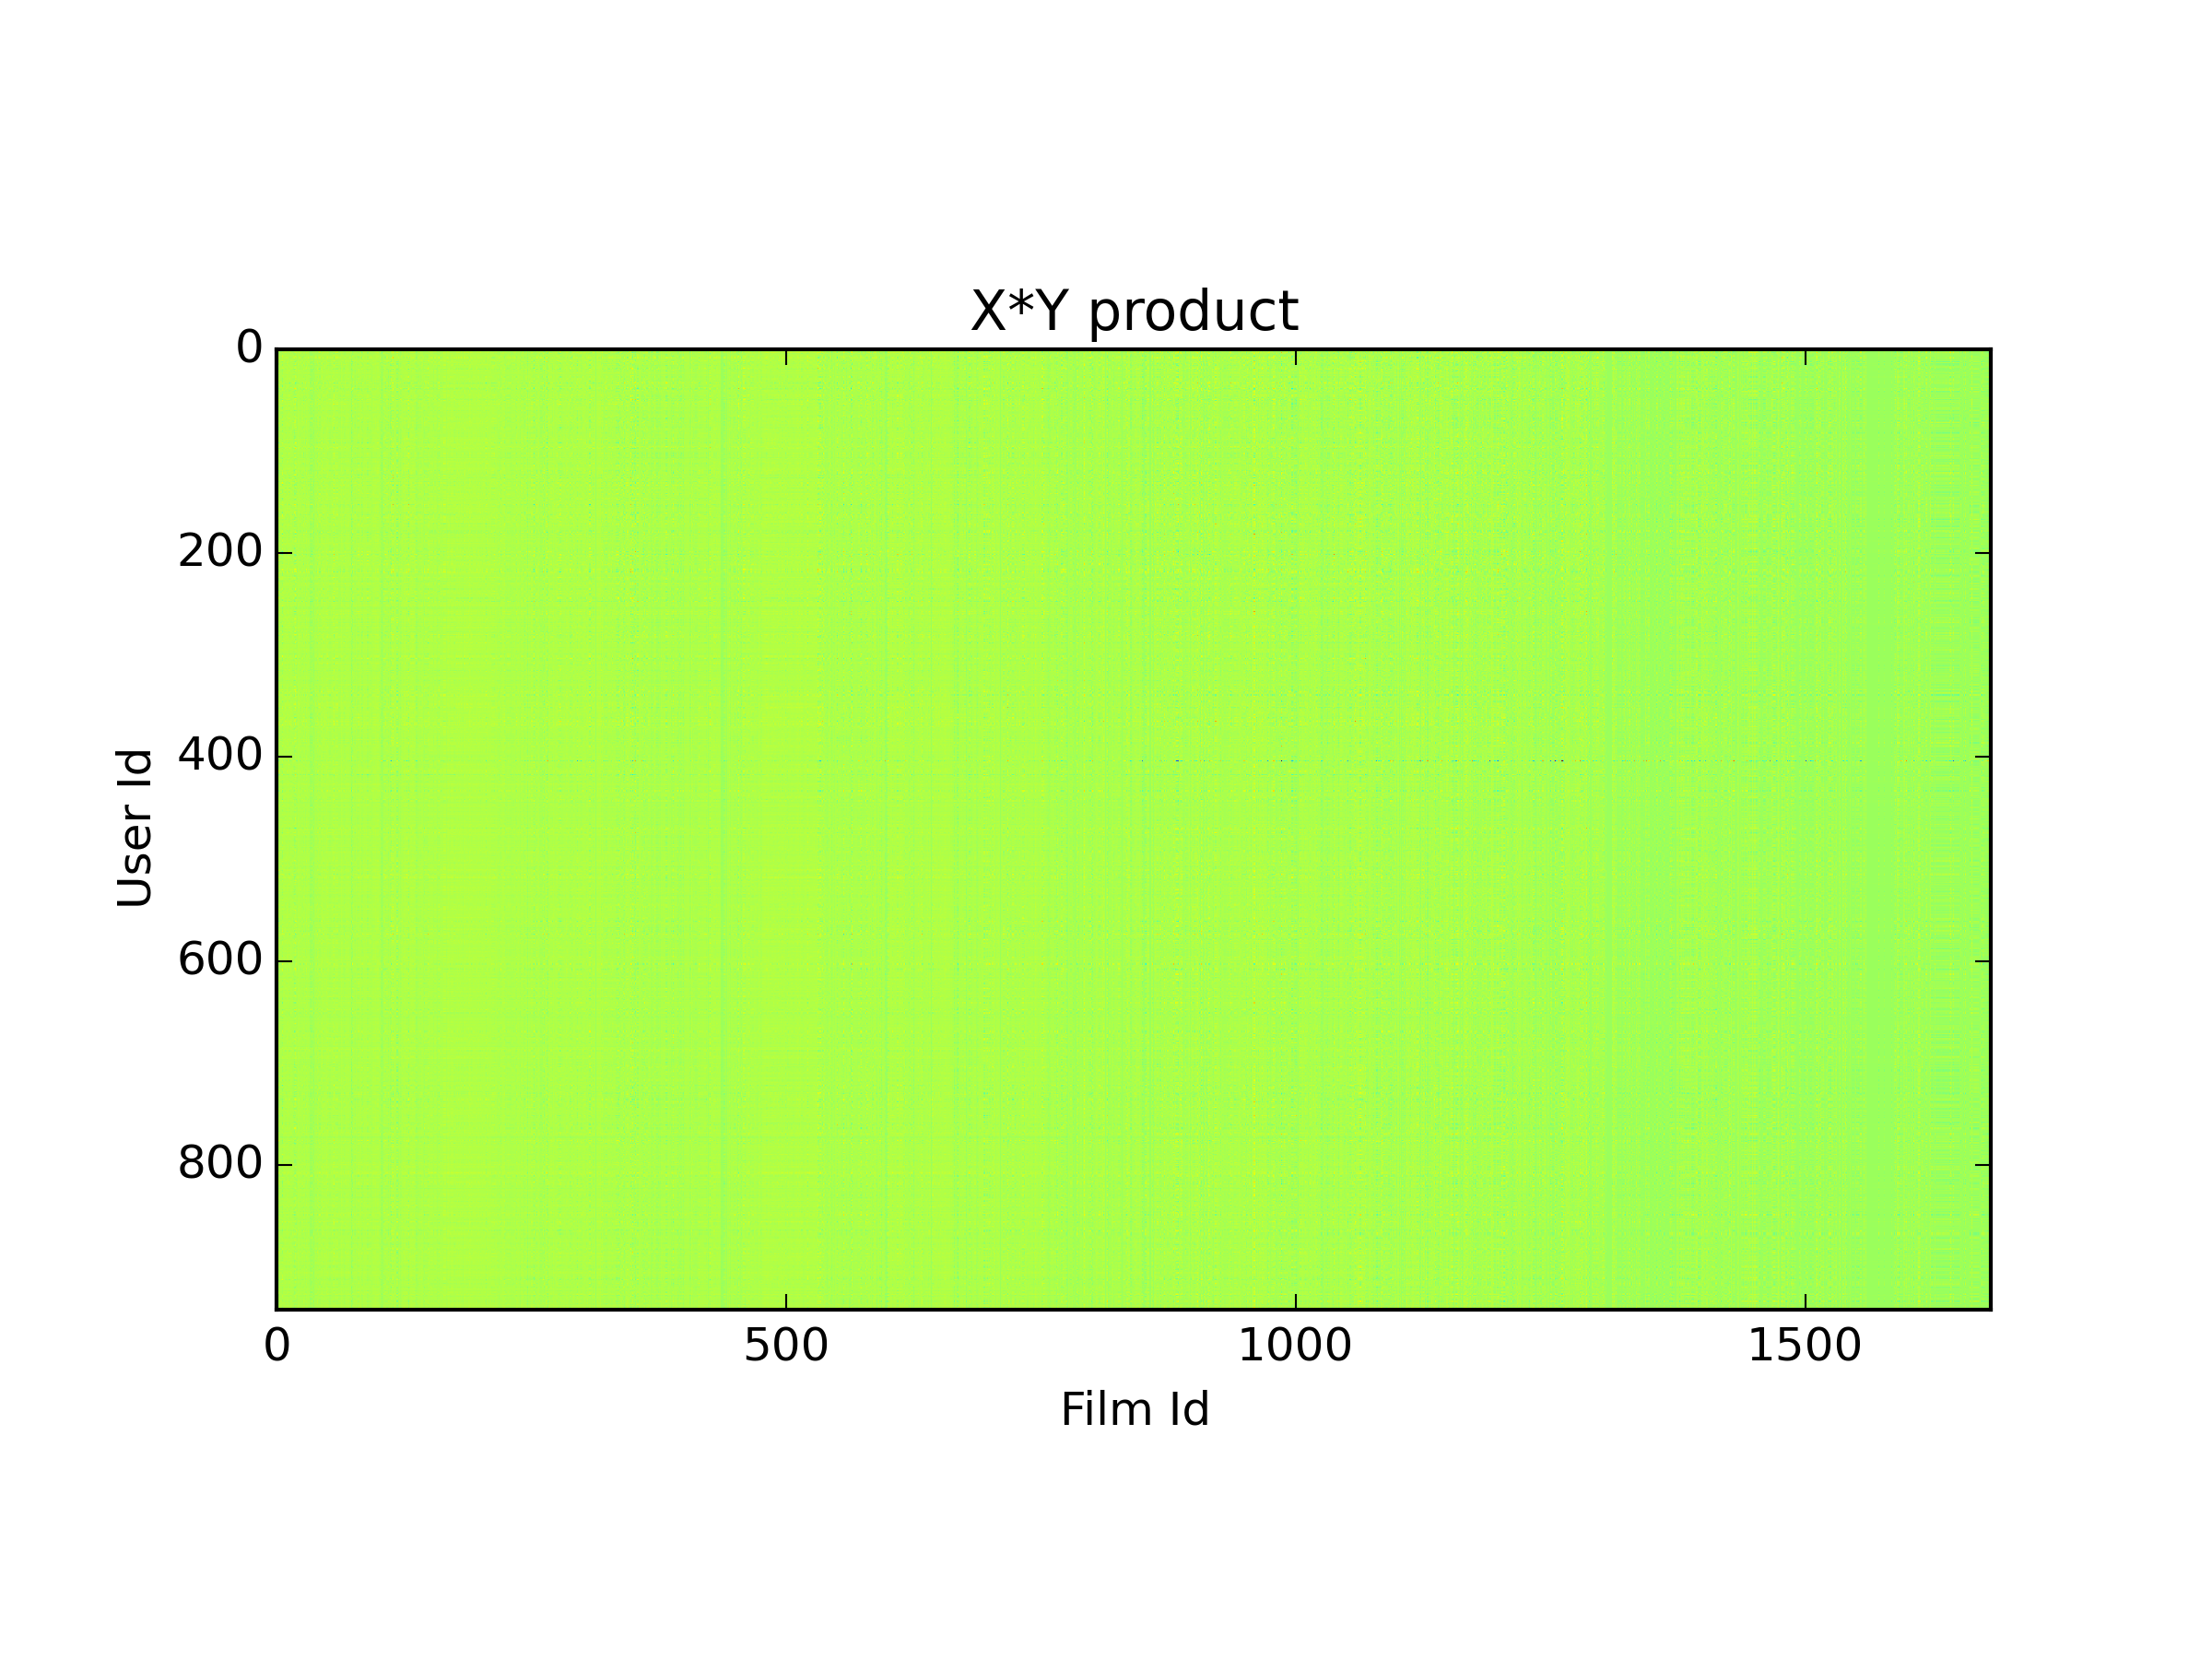
\includegraphics[scale=0.2]{it10-k12-l2.png}}
\end{tabular}
\caption{Pour k=12, $\lambda$=0.02}
\end{table}

\begin{table}[h]
\begin{tabular}{cccc}
\subfloat[X*Y à la $1^{ere}$ itération]{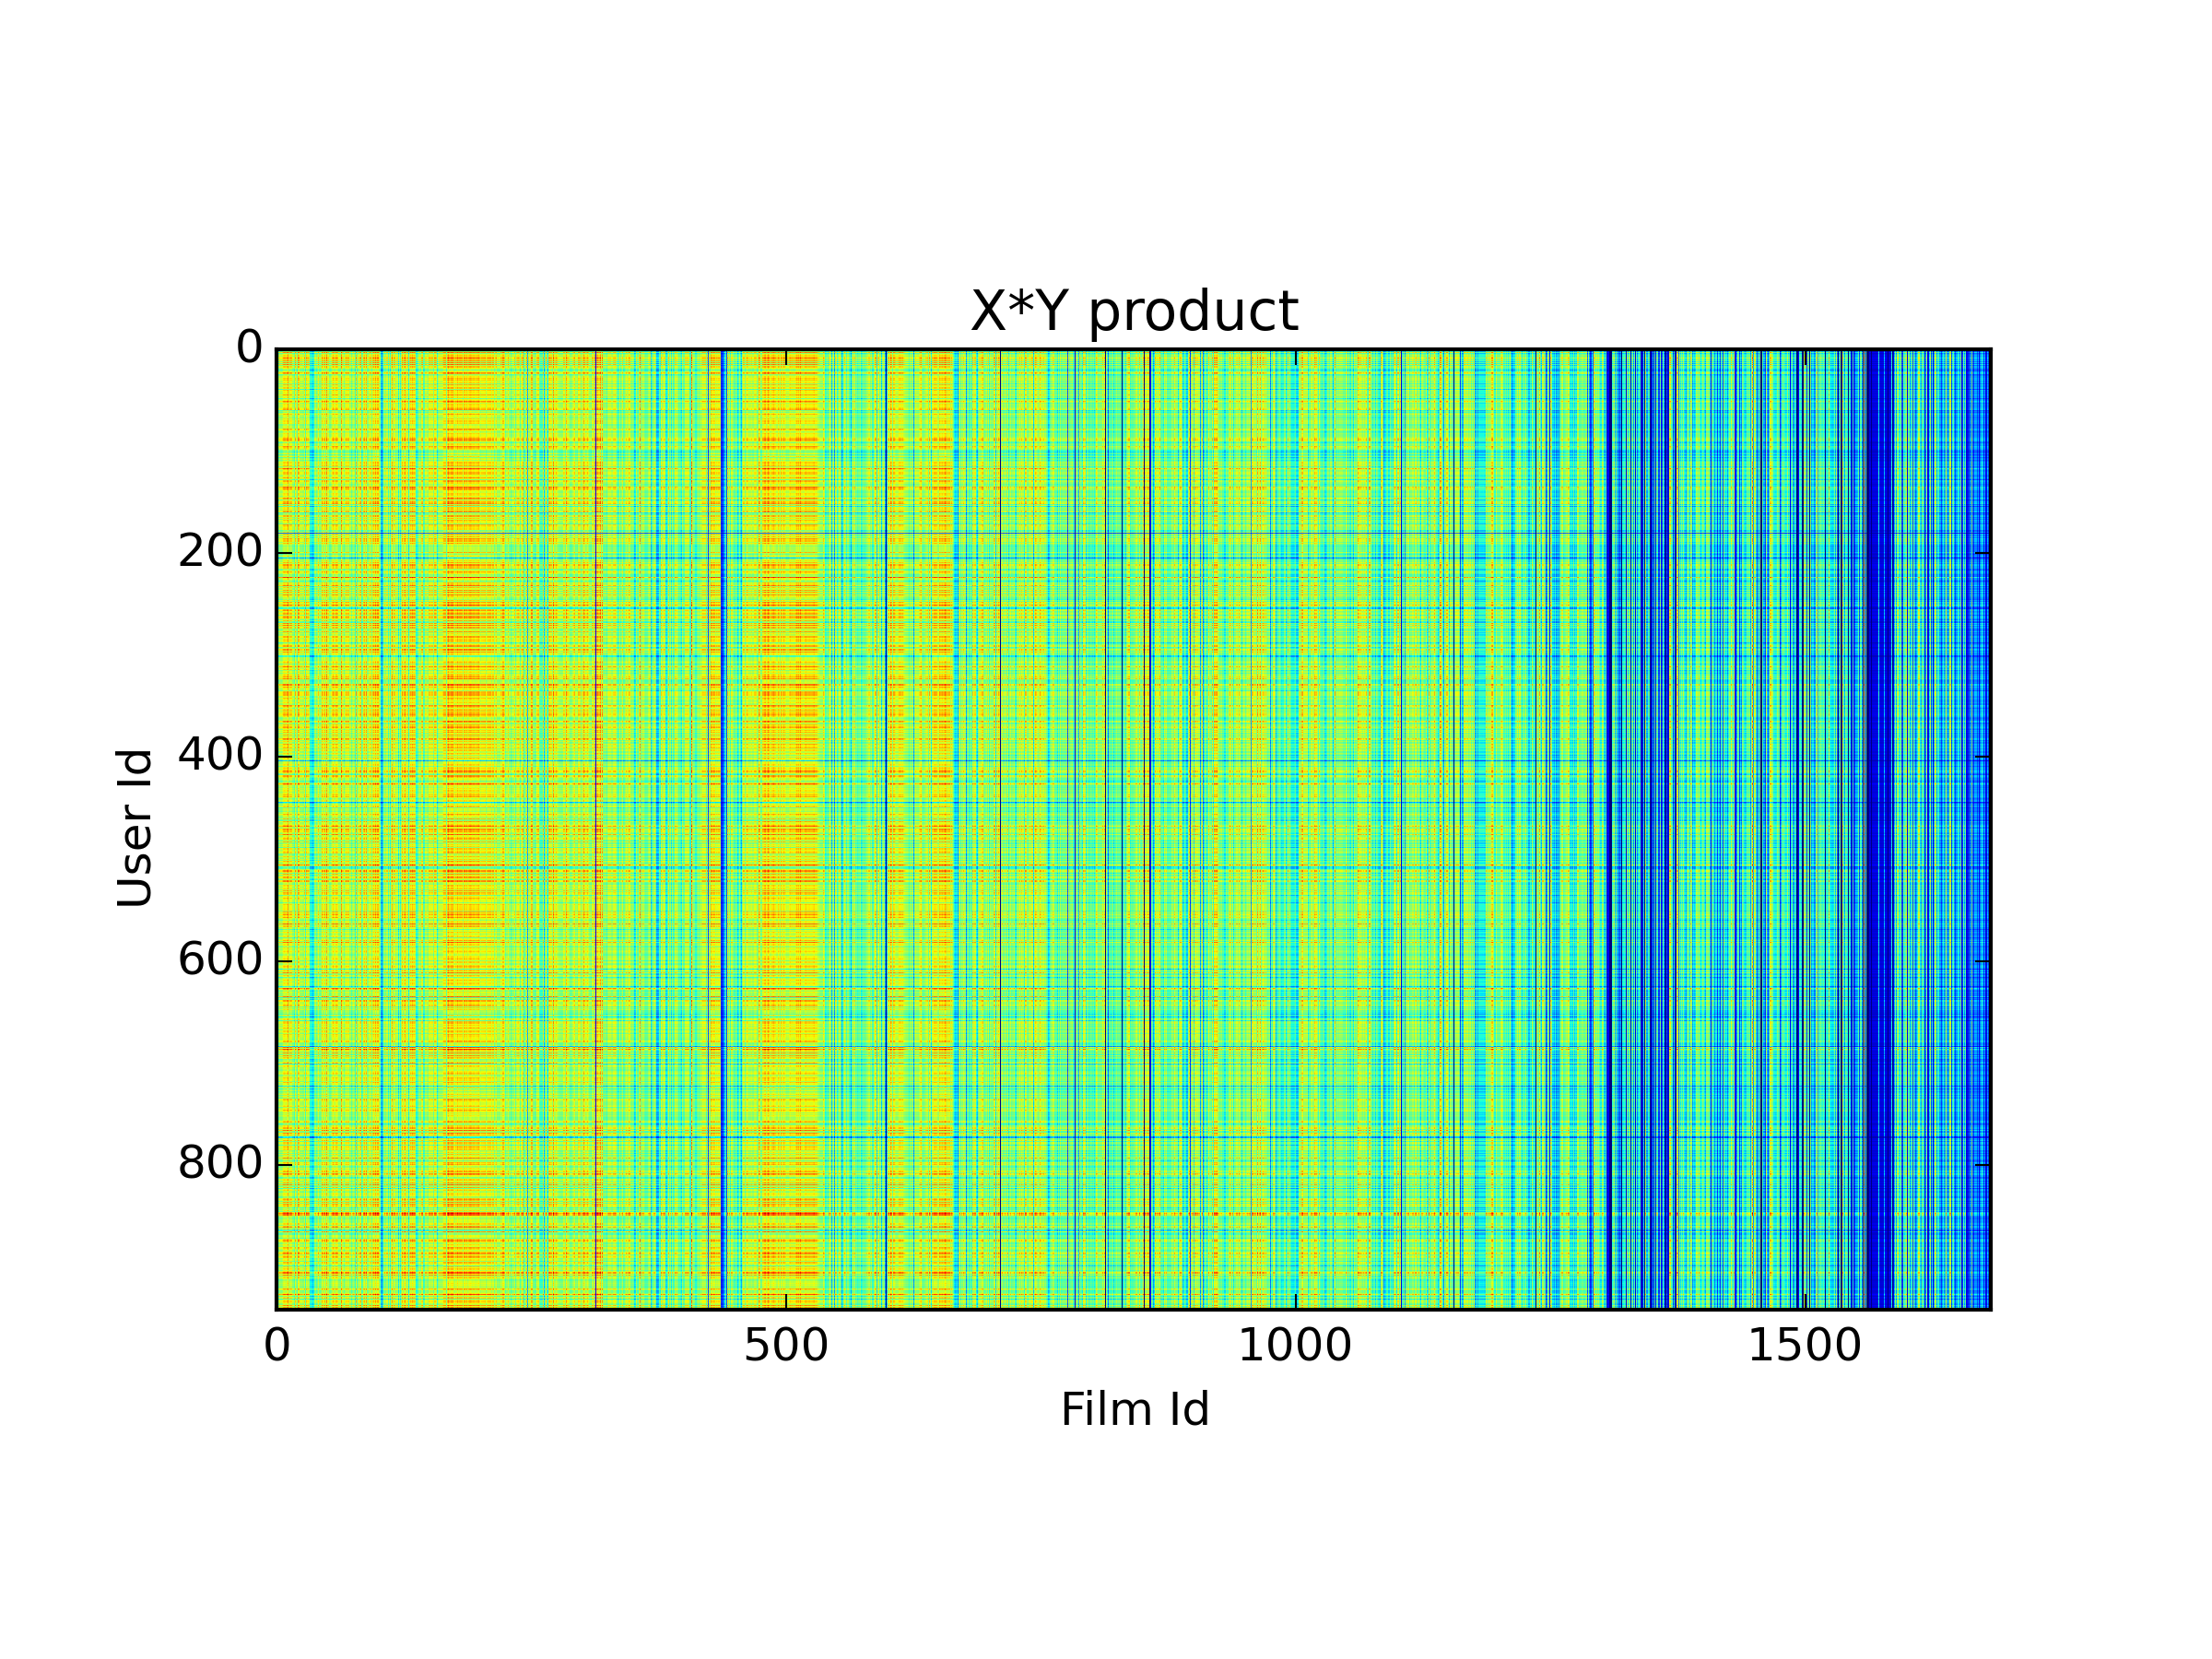
\includegraphics[scale=0.2]{it1-k12-l80.png}}
&
\subfloat[X*Y à la $2^e$ itération]{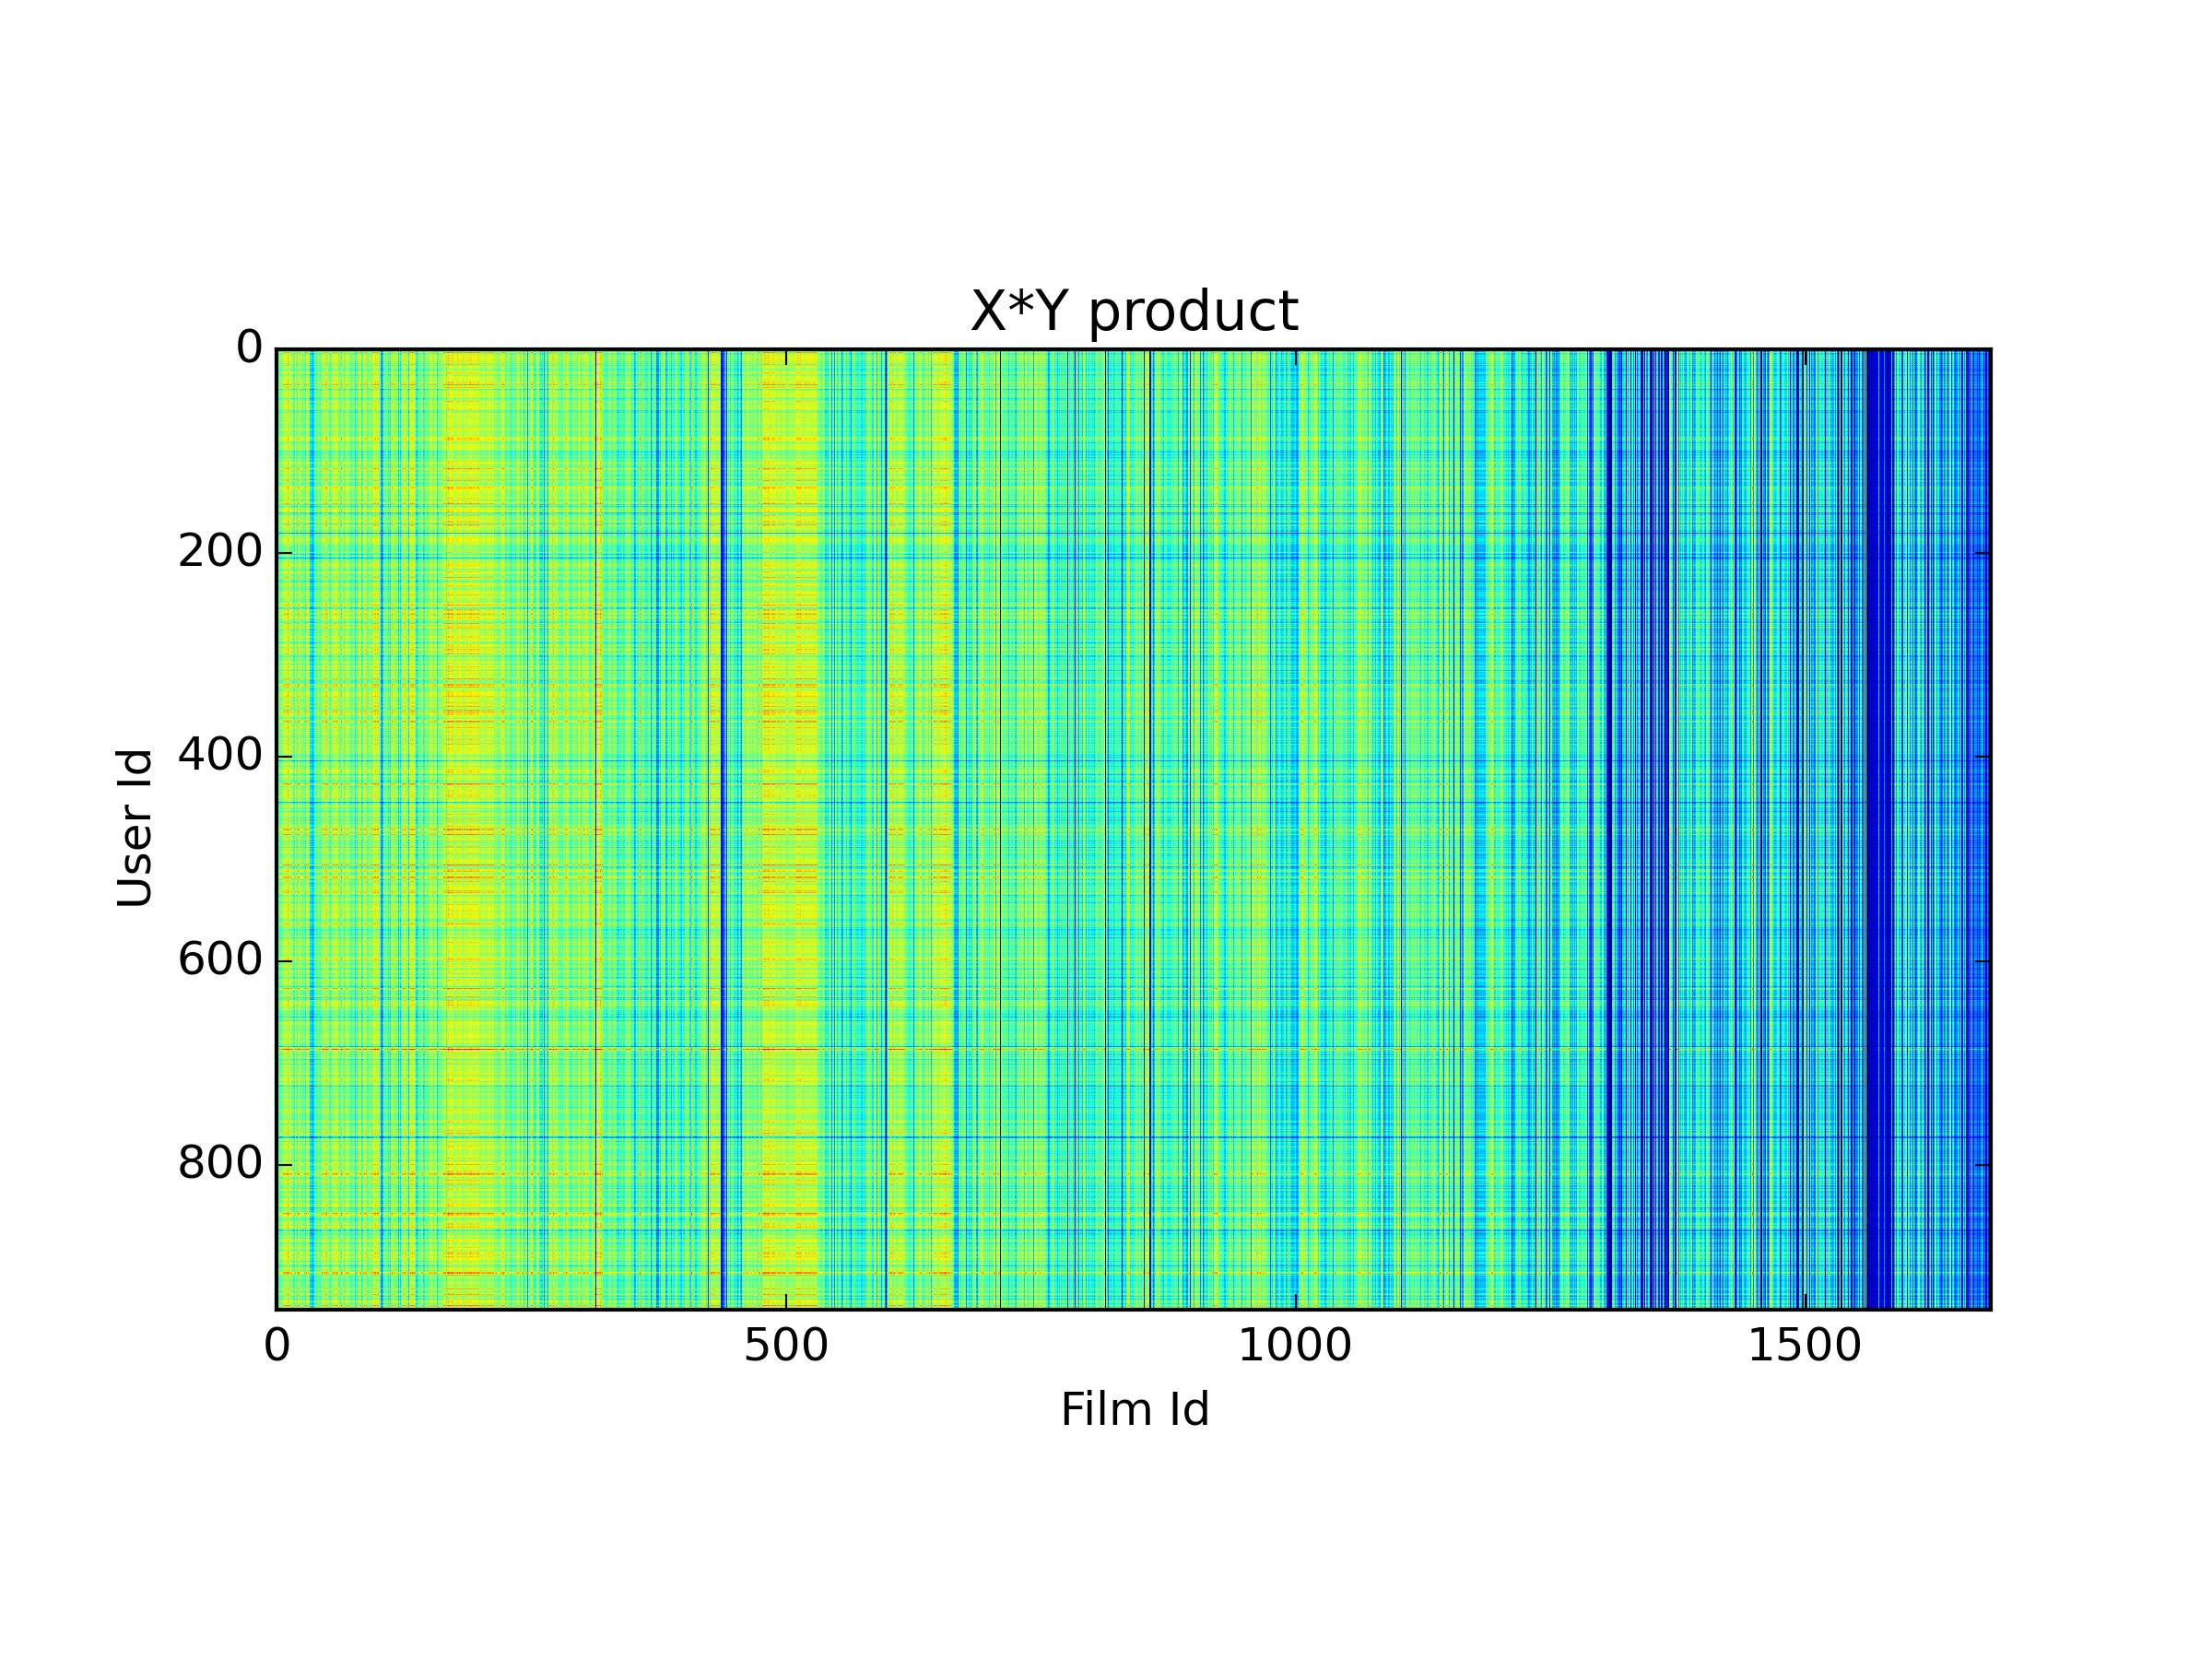
\includegraphics[scale=0.2]{it2-k12-l80.png}}
&
\subfloat[X*Y à la $10^e$ itération]{\includegraphics[scale=0.2]{it10-k12-l80.png}}
&
\subfloat[X*Y à la $50^e$ itération]{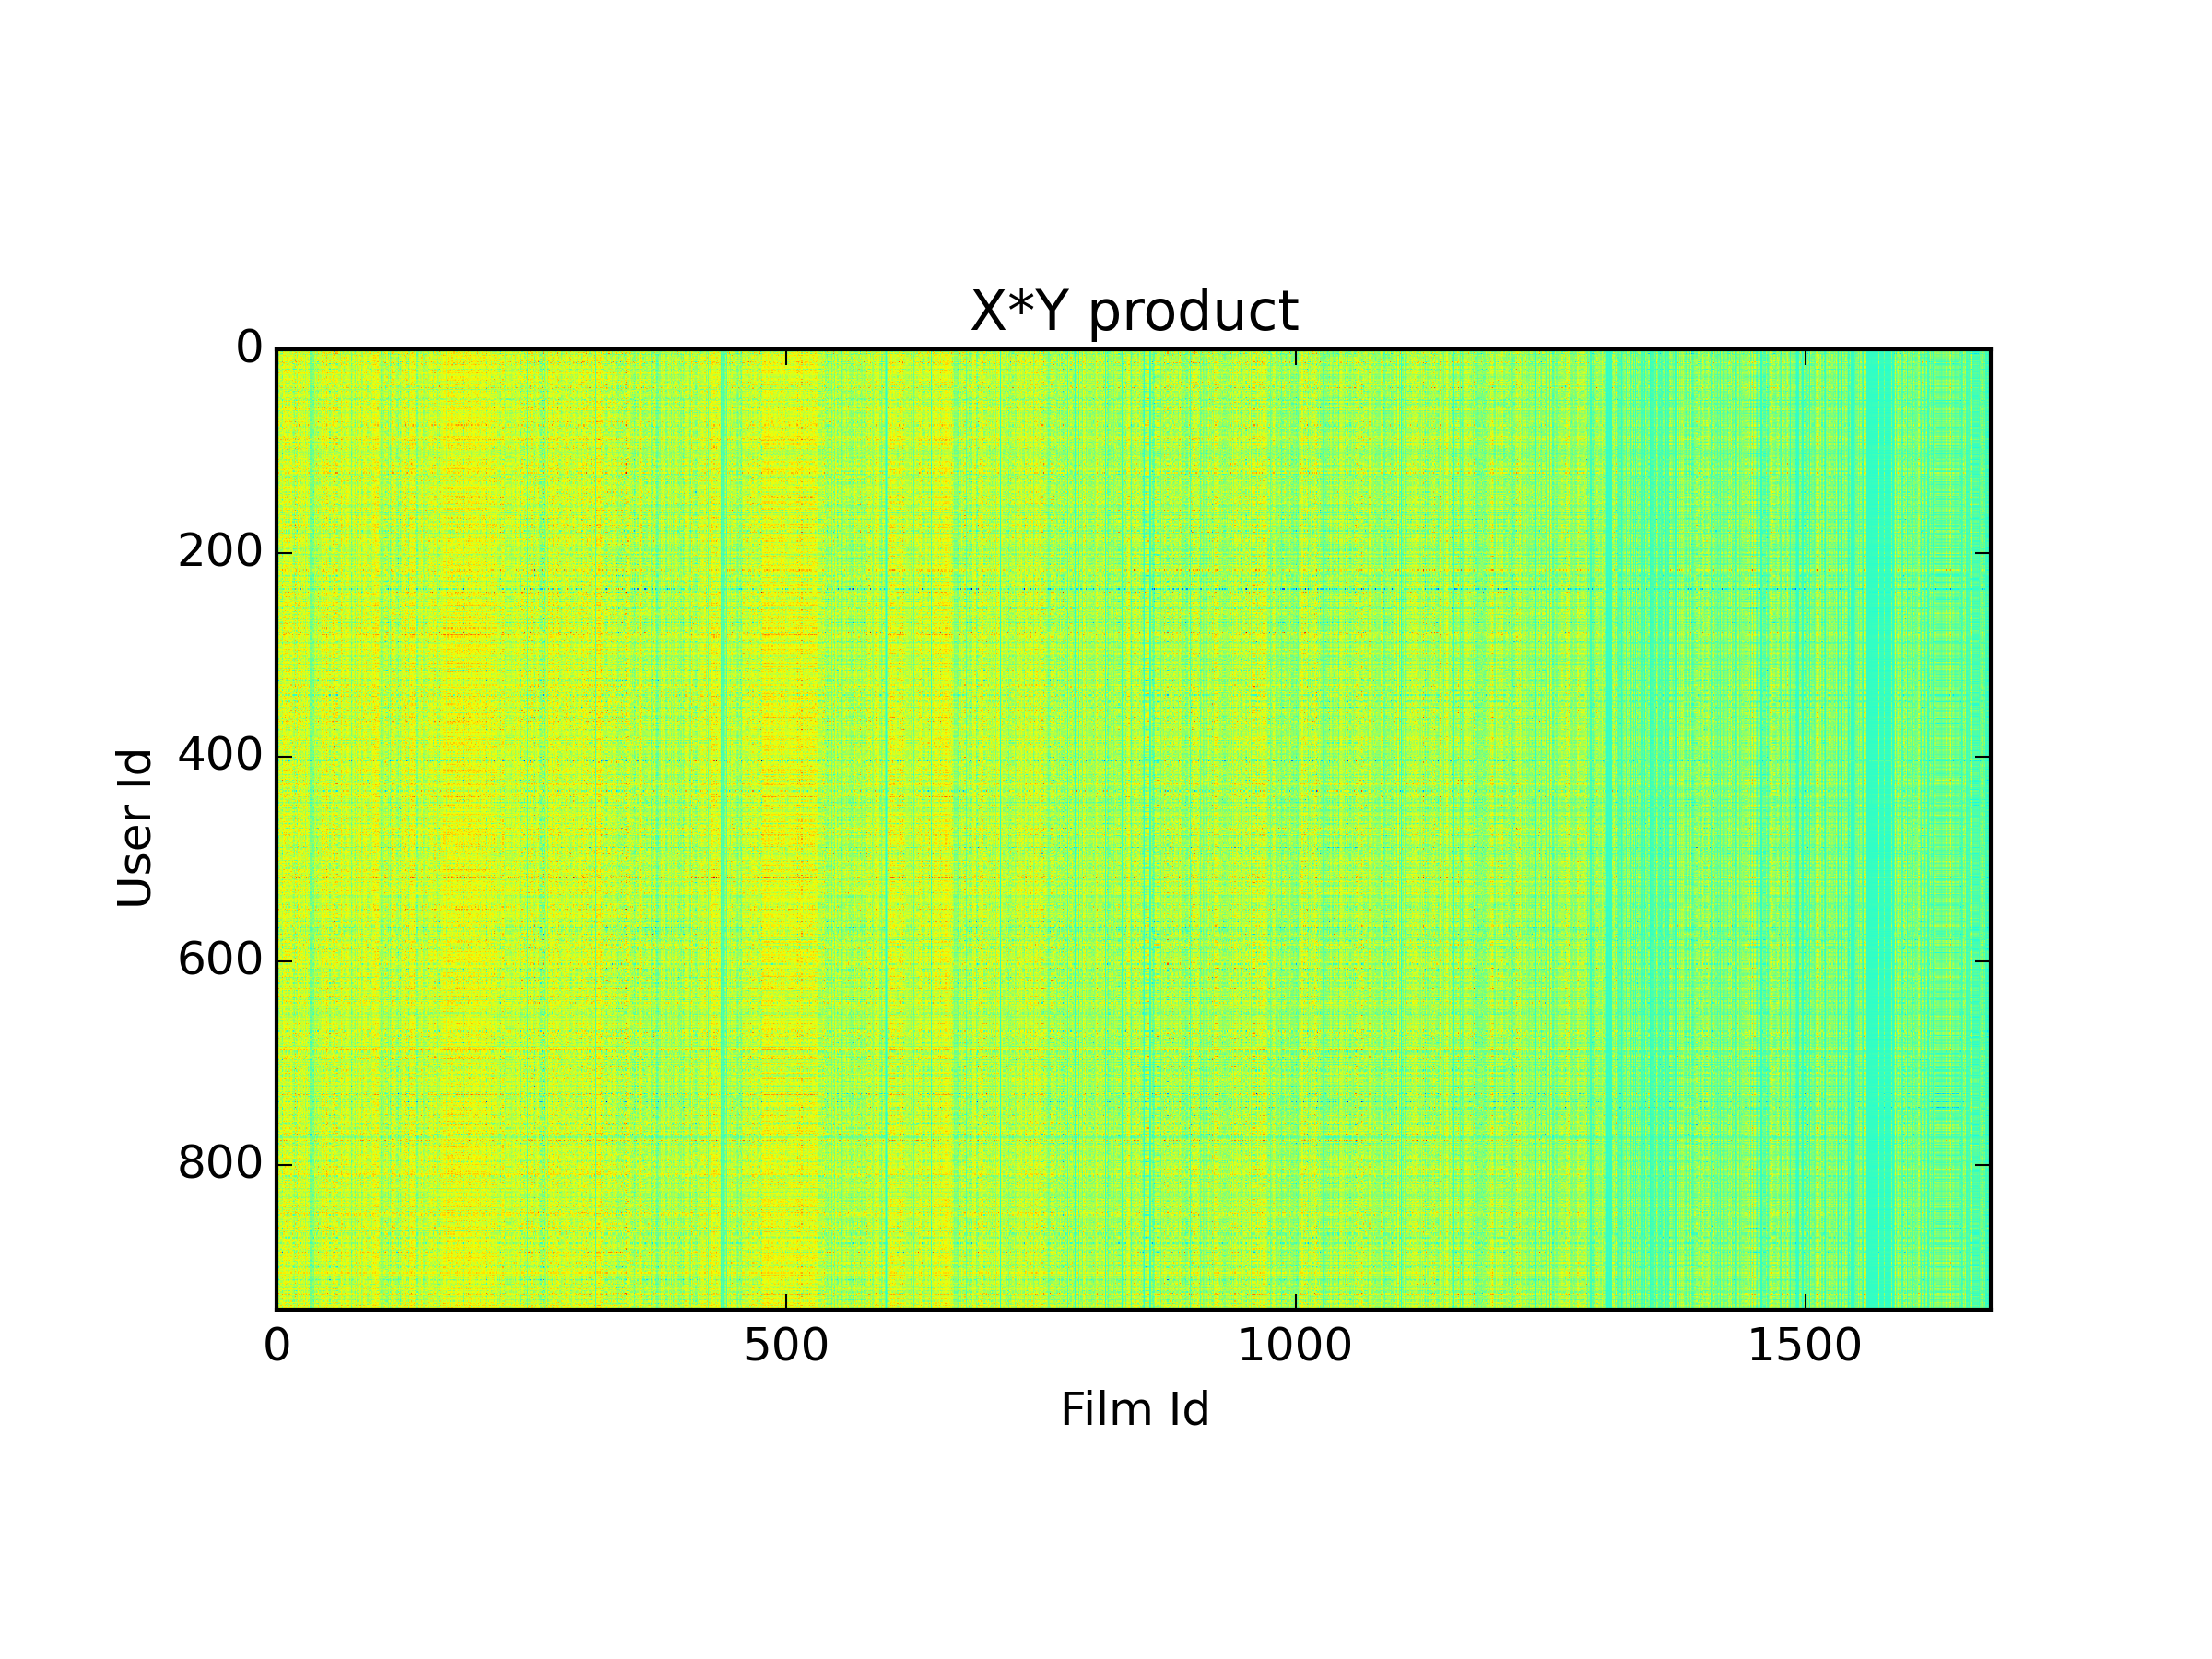
\includegraphics[scale=0.2]{it35-k12-l80.png}}
\end{tabular}
\caption{Pour k=12, $\lambda$=0.80}
\end{table}
\end{document}
